\documentclass[a4paper,openright]{book}

\usepackage [utf8]{inputenc}
\usepackage [english]{babel}					%Lingua e sillabazione italiana
\usepackage {graphicx}						%Immagini
\usepackage {subfig}
\usepackage {caption}						%Didascalie
\usepackage {wrapfig}						%Testo che avvolge un'oggetto
\usepackage {amsfonts, amsmath, amssymb, esint, mathrsfs}	%Font e simboli matematici
\usepackage {amsthm}						%Definizioni e teoremi
\usepackage {mathtools}						%Comandi abs e norm	definiti sotto
\usepackage {fancyhdr}						%Abstract in {book}
\usepackage {booktabs}						%Tabelle
\usepackage {hyperref}						%Collegamenti rossi e verdi
\usepackage {mhchem}						%Per il typesetting di formule chimiche - comando \ce{formula}
\usepackage {siunitx}
\usepackage {pstricks}
%\usepackage[paperwidth=169mm, paperheight=239mm]{geometry}
\usepackage[style=authoryear,
            maxcitenames=1,
            hyperref,
            isbn=false,
            url=false,
            doi=false,
            eprint=false,
            firstinits=true,
            backend=biber]{biblatex}

%%%%%%%%%%%% Font Alternativi %%%%%%%%%%%%%%%%%%%
%\usepackage{mathpazo}
%\usepackage{mathptmx}
%\usepackage{fourier}
%\usepackage{pxfonts}

\newcommand{\mail}[1]{\href{mailto:#1}{\texttt{#1}}}

\usepackage {listings}						%Per il codice
	\lstset {
		language=C++,
		inputencoding=utf8,
		numbers=left,
		extendedchars=\true,
		showstringspaces=\false,
		basicstyle=\small\ttfamily,
		keywordstyle=\color{darkgreen}\bfseries,
		commentstyle=\color{blue},
		stringstyle=\color{fuxia},
	}

\usepackage {color}							%Definire colori
	\ifx\color@rgb\@undefined\else
		\definecolor{darkgreen}{rgb}{0,0.55,0}
		\definecolor{fuxia}{rgb}{1,0,0.98}
	\fi



\makeatletter								%Gestione dei bookmark nel pdf
\newcommand\deftoclevel[2][chapter]{%
\expandafter\renewcommand\csname toclevel@#1\endcsname{#2}}
\makeatother		%il comando \deftoclevel{-1} riporta il bookmark fuori di un livello

% \usepackage {fancyhdr}						%Testatine ed Abstract in {book} come nella tesi liceo
% \fancyhf{}
% \fancyhead[RO,LE]{\thepage}
% \fancyhead[LO]{\nouppercase{\slshape\rightmark}}
% \fancyhead[RE]{\nouppercase{\slshape\leftmark}}
% \pagestyle{fancy}
% \setlength{\headheight}{13.6pt}

\renewcommand{\epsilon}{\varepsilon}		%Definizione delle lettere greche per la tipografia italiana
\renewcommand{\theta}{\vartheta}
%\renewcommand{\rho}{\varrho}
\renewcommand{\phi}{\varphi}

\DeclareMathOperator{\NN}{\mathbb{N}}
\DeclareMathOperator{\RR}{\mathbb{R}}
\DeclareMathOperator*\argmin{arg\,min}
\DeclareMathOperator*\argmax{arg\,max}
\DeclareMathOperator\tr{tr}
\DeclareMathOperator\sym{sym}
\DeclareMathOperator\skw{skw}
%\DeclareMathOperator\grad{grad}
\DeclareMathOperator\grad{\nabla}
\DeclareMathOperator\rot{rot}
\DeclareMathOperator\curl{curl}
\DeclareMathOperator\divergence{div}
\renewcommand{\div}{\divergence}

\def\d{\,\,\textrm{d}}				%il differenziale in testo dritto


\DeclarePairedDelimiter{\abs}{\lvert}{\rvert}
\DeclarePairedDelimiter{\norm}{\lVert}{\rVert}

%\def\wto{\overset{w}{\to}}
\def\wto{\rightharpoonup}
\def\vec{}
\def\vec{\mathbf}

\relpenalty=9999				%evita che le formule inline siano spezzate da fineriga QUASI sempre
\binoppenalty=9999				%impostare a 10000 per evitare SEMPRE

\newcommand{\<}{\langle}
\renewcommand{\>}{\rangle}

\theoremstyle{definition}					%Dichiarazione di teoremi e definizioni
\newtheorem{definizione}{Definizione}

\theoremstyle{plain}
\newtheorem{teorema}{Teorema}
\newtheorem*{teorema_bis} {Teorema}
\newtheorem{proposizione}{Proposizione}

\addbibresource{/home/mleoni/Papers/library.bib}

\graphicspath{{img/rfa/}}

\title{Finite elements simulation of turbulent flows: computations and
applications}
\author{Massimiliano Leoni}
\date{}

\begin{document}

  \frontmatter
  \maketitle

  \tableofcontents

  \mainmatter

  \part{Introductory chapters}
  \chapter{Introduction}
\label{cha_introduction}

I have always been interested in mathematics, and I have always been fascinated by science.
I find it obvious and surprising, at the same time, that I found myself seizing any opportunity to steer my own research focus in the direction of applications of mathematics to problems in science and technology.
The field of numerical simulations offers the perfect ground to grow and nurture my passions into real scientific progress, being at the intersection of mathematics, a variety of applied sciences, and computer programming -- a dark art I find difficult to resist.
This is the gist of this thesis: I will take my reader through advances in simulation technology and applications to a challenging biomedical problem, in an attempt to celebrate how Mathematics truly is \emph{the art of giving the same name to different things}.
Let us dive in.

Given the wide range of topics this thesis necessarily covers, the present
chapter briefly recalls the fundamental ideas of the building blocks
upon which later chapters are built.
This is intended to give a high-level understanding of the
concepts to readers coming from different backgrounds and does not aim
to be a complete introduction to the corresponding topics.
I assume only basic knowledge of calculus, mechanics and computer
science on the reader's side.

\section{Real Unified Continuum Simulation: predictive fluid and solid dynamics}
\label{sec_cfd}
The two key scientific frameworks which enable the breakthrough
results in the thesis are: Digital Math [ref] and Real Unified Continuum
Simulation (RUC) [ref]. Digital Math is the foundation of modern
science based on constructive digital mathematical computation, where
the source code in FEniCS symbolic form and computational results are
digital scientific objects - allowing reproducibility and
falsifiability. Real Unified Continuum Simulation is a Direct FEM
Simulation of first principles allowing general phenomena such as
multiphase fluid-structure interaction (FSI), general interface
motion, implicit contact, fracture, plasticity, etc., The methodology
also allows application of Direct duality-based adaptive error
control. RUC is a generalization of the Unified Continuum framework
which was developed previously in [ref].

Fluid dynamics is a very vast field.
With basic ideas going back to Euler, fluid dynamics has since become a
central part of mechanical, aerospace and civil engineering providing
useful insight into how to build aeroplanes, cars and bridges but also
heart valves and nuclear reactors.
Despite being so important, some questions in fluid mechanics still do not
have a satisfactory answer, one such example being turbulence, one of the last few
open problems in classical mechanics that still eludes our
comprehension.
Part of the issue is that turbulence, the disordered and chaotic motion that fluids
undergo when friction between particles dominates their diffusion, is too
expensive to fully simulate in a computer because the features the flow
develops are too fine for the resolution power of modern supercomputing
clusters.

In this context I will only address incompressible, viscous fluid
dynamics.
The word \emph{incompressible} refers to the fact that the fluid at hand
does not show any compressibility effect, meaning that its density
remains constant in time.
This is a good approximation for all liquids and for gases under appropriate conditions, such as air at relatively low speeds and Mach number up to \num{0.3}.
The word \emph{viscous} means that the particles of the fluid do not slip
past each other frictionlessly, but instead experience friction from each
other and can drag each other around.
This is a reasonable assumption for almost all fluids that we encounter
in engineering practice.

The most famous equations of fluid dynamics are the Navier-Stokes
equations, a system of two equations encoding conservation of mass and momentum.
For viscous, incompressible fluids, the former reads
\begin{equation}
  \div \vec{u} = 0
  \label{eq_mass}
\end{equation}
while the latter reads
\begin{equation}
  \rho\partial_{t} \vec{u} - \mu \Delta \vec{u} + \rho(\vec{u} \cdot \grad)
  \vec{u} - \grad p = \vec{f}
  \label{eq_momentum}
\end{equation}
where \(\vec{u}\) is the fluid velocity, \(\mu\) is the dynamic
viscosity, \(p\) is the pressure, \(\rho\) is the density and \(\vec{f}\)
represents the external forces such as gravity.

The mass conservation equation \eqref{eq_mass} expresses the fact that
the fluid is incompressible: a zero-divergence velocity field means,
intuitively, that in any given point as much fluid is arriving as is
leaving, implying that the total volume of the fluid remains constant.
The momentum conservation equation \eqref{eq_momentum} is a suitable
reformulation of Newton's second law that forces \(F\) applied to matter change
its momentum \(Q\) according to
\begin{equation}
  F = \dot Q;
  \label{eq_newtonSecondLaw}
\end{equation}
in the case of Equation~\eqref{eq_momentum}, the momentum is \(\dot
{\rho \vec{u}} = \rho \partial_{t} \vec{u} + \rho (\vec{u} \cdot \grad)
\vec{u}\) and the applied forces are \(\div \sigma(\vec{u}, p) = \mu
\Delta \vec{u} + \grad p + \vec{f}\), where \(\sigma(\vec{u}, p)\) is the
stress tensor \(\sigma(\vec{u}, p) = 2 \mu \sym\grad \vec{u} - pI\) and \(\sym A = \frac{A + A^t}{2}\) is the symmetric part of \(A\);
Equation~\eqref{eq_momentum} can then be compactly expressed as
\begin{equation}
  \dot {\rho \vec{u}} = \div \sigma(\vec{u}, p),
  \label{eq_momentumDerivatives}
\end{equation}
beautifully expressing how derivatives capture the essence of our world.

For incompressible fluids, where density is constant, it is common to
normalise the equations choosing a domain of unitary characteristic
length and a flow of unitary characteristic speed, together with a
unitary density.
After these changes of variables, but without changing notation for
convenience, the equations read
\begin{equation}
  \left\{
    \begin{aligned}
      &\partial_{t} \vec{u} - \nu \Delta \vec{u} + (\vec{u} \cdot \grad)
        \vec{u} - \grad p = \vec{f} \\
      &\div \vec{u} = 0
    \end{aligned}
  \right.
  \label{eq_ns}
\end{equation}
where now \(\nu = \frac{\mu}{\rho}\) is the kinematic viscosity and \(p\)
and \(\vec{f}\) have been implicitly divided by the density.
The only parameter left, \(\nu\), is the ratio of the dynamic viscosity
to the density and models the flow based on how strong diffusion effects
are compared to inertial effects, and it is so important that its inverse
is given the name of \emph{Reynolds number} \(Re = \nu^{-1}\).
The Reynolds number, being the only nondimensional group left in
Equation~\eqref{eq_ns}, determines the features of the resulting
solution: in a flow with small Reynolds number, particles diffuse much
faster than they drag each other around, resulting in smooth, laminar
velocity profiles, whereas in a flow with high Reynolds number the
opposite happens, and the velocity profile is turbulent and chaotic.

It should be noted that the real definition of the Reynolds number is
\begin{equation}
  Re = \frac{LU}{\nu}
  \label{eq_reynolds}
\end{equation}
with \(L\) and \(U\) a characteristic length and speed of the system,
such as, for example for the case of flow past a wing profile, the wing length and
the far-field velocity.
The definition I gave above keeps into account that
Equation~\eqref{eq_ns} was normalised such that \(L = 1\) and \(U = 1\).


\section{Finite elements}
\label{sec_fem}
The Finite Elements Method, or FEM for brevity, is a technique to approximate the solution to partial differential equations, or PDEs.
This method is very popular in many fields of engineering due to its versatility and its ability to gracefully handle complex geometries, typical of practical applications.

I will now briefly illustrate the principles of the Finite Elements Method on the very famous Poisson equation
\begin{equation}
  \begin{cases}
   -\Delta u = f, &\text{ in } \Omega \\
   u = 0, &\text{ on } \Gamma_D \\
   \partial_{n} u = 0, &\text{ on } \Gamma_N \\
  \end{cases}
  \label{eq_poisson}
\end{equation}
where \(\Omega \subset \mathbb{R}^n\) is an open, connected, regular domain, \(\Gamma_D\) and \(\Gamma_N\) are two disjoint subsets of \(\partial \Omega\), such that \(\Gamma_D \cup \Gamma_N = \partial \Omega\), where Dirichlet and Neumann boundary conditions are applied, respectively.
Here, \(u = u(\vec{x})\) and \(f = f(\vec{x})\) are functions on
\(\Omega\).
Considering non-homogeneous Dirichlet and Neumann boundary conditions just adds
inessential details to the following discussion without changing the
ideas, so we will not be concerned with it here\footnote{Basically, you
can reduce non-homogeneous boundary conditions to homogeneous ones by an
appropriate change of variables.}.
Finally, \(\Delta = \div \grad\) is the Laplace operator and \(\partial_{n}\) is the normal derivative operator, defined as \(\partial_{n} u = \grad u \cdot \vec{n}\) with \(\vec{n}\) the unit normal.

Some background is required before jumping into the FEM formulation of Equation~\eqref{eq_poisson}.
Equation~\eqref{eq_poisson}, in its classical interpretation, means that we are looking for a function \(u\) that satisfies it in every point \(\vec{x}\) in the closure of the domain, \(\overline\Omega\).
Such a function needs to be twice continuously differentiable in \(\Omega\) and continuous up to the boundary, or \(u \in C^2(\Omega) \cap C^0(\overline\Omega)\) for short, otherwise it would not make sense to talk about the Laplacian of \(u\).

This requirement turns out to be too strict for many practical applications, resulting in ill-posed problems, meaning equations that do not have a solution but that describe phenomena that do exist.
A way to overcome this is to relax the above requirement by choosing a test function \(v\) in an appropriate function space \(X\), multiply Equation~\eqref{eq_poisson} by it and integrate by parts.
Keeping in mind that, for a scalar function \(w\) and a vector function \(\vec{\psi}\), the Leibniz rule reads
\begin{equation}
  \div(w \vec{\psi}) = w \div \vec{\psi} + \vec{\psi} \cdot \grad w
  \label{eq_leibniz}
\end{equation}
and using the Stokes theorem
\begin{equation}
  \int_\Omega \div \vec{\psi} = \int_{\partial\Omega} \vec{\psi} \cdot \vec{n}
  \label{eq_stokes}
\end{equation}
Equation~\eqref{eq_poisson} can be rewritten as
\begin{equation}
  \int_\Omega \grad u \cdot \grad v = \int_\Omega f v + \int_{\partial\Omega} \partial_{n} u \cdot v.
  \label{eq_poissonWeakNoBC}
\end{equation}
The improvement is that this equation now makes sense under less strict
conditions, namely that the integrals it features converge.
We can recover the boundary conditions in Equation~\eqref{eq_poisson} by
modifying the boundary term in Equation~\eqref{eq_poissonWeakNoBC},
splitting it into two integrals over \(\Gamma_D\) and \(\Gamma_N\),
substituting \(\partial_{n} u = 0\) in the latter, which disappears, and requiring the test function \(v\) to
be zero on \(\Gamma_D\), making the first term disappear as well.
The final result is
\begin{equation}
  \int_\Omega \grad u \cdot \grad v = \int_\Omega f v.
  \label{eq_poissonWeakNoForall}
\end{equation}
We can now claim that a function \(u\) satisfies
Equation~\eqref{eq_poisson} if it satisfies
Equation~\eqref{eq_poissonWeakNoForall} for all test functions \(v \in X\).
This claim is an approximation, which is good only if the chosen space
\(X\) is sufficiently large.
We note that the opposite claim is obviously true.
The choice of \(X\) requires some knowledge of Functional Analysis; in
this text I will only report that a natural choice is
\(H^1_{\Gamma_D}(\Omega)\), the set of functions \(u\) that satisfy
\[
  \int_\Omega u^2 < +\infty \qquad \text{and} \qquad \int_\Omega \norm*{\grad u}^2 < +\infty
\]
and that are zero\footnote{In an appropriate sense.} on \(\Gamma_D\).
With this choice, it is also natural to look for a solution \(u\) in the
same space.

We finally have what is called a \emph{weak formulation} of
Equation~\eqref{eq_poisson}: find \(u \in H^1_{\Gamma_D}(\Omega)\) such
that
\begin{equation}
  \int_\Omega \grad u \cdot \grad v = \int_\Omega f v \qquad \forall v
  \in H^1_{\Gamma_D}(\Omega).
  \label{eq_poissonWeak}
\end{equation}
The left hand side and the right hand side of Equation~\eqref{eq_poissonWeak} define a
bilinear form \(a : H^1_{\Gamma_D}(\Omega) \times H^1_{\Gamma_D}(\Omega)
\mapsto \mathbb{R}\) and a linear form \(L : H^1_{\Gamma_D}(\Omega)
\mapsto \mathbb{R}\), respectively.
The equation is often expressed in the more compact form: find \(u \in
H^1_{\Gamma_D}(\Omega)\) such that
\begin{equation}
  a(u, v) = L(v)  \qquad \forall v \in H^1_{\Gamma_D}(\Omega).
  \label{eq_poissonForms}
\end{equation}

We are now ready to give a FEM formulation of
Equation~\eqref{eq_poissonWeak}.
The idea is to define a finite dimensional approximation of \(X\), which
is an infinite dimensional space, so that
we can enter the computation in a computer and get an output.
Given a simplicial mesh \(\mathcal{T}_h\) -- a mesh made of triangles or tetrahedra --
describing \(\Omega\), we can use, for example, the space \(V_h =
\mathbb{P}^1\) of functions
that are linear on every cell of \(\mathcal{T}_h\) and globally
continuous (and incorporate the Dirichlet boundary condition).
The dimension of this space is the number \(N\) of the vertexes in the mesh, so
it is finite dimensional.

Applying this approximation, our problem now reads: find \(u_h \in V_h\)
such that
\begin{equation}
  \int_{\Omega} \grad u_h \cdot \grad v_h = \int_{\Omega} f v_h \qquad
  \forall v_h \in V_h
  \label{eq_poissonGalerkin}
\end{equation}
The final step to make the solution computable is to observe that
Equation~\eqref{eq_poissonGalerkin} is true if and only if it is true for
a set of functions \(\{\phi_i\}_i\) that form a basis of \(V_h\);
incidentally, being \(u_h \in V_h\), it can also be expressed as a linear
combination of the functions \(\{\phi_i\}_i\) with unknown coefficients
\(\{u_h^i\}_i\), called \emph{degrees of freedom} in this context:
\[
  u_h = \sum_{i=1}^N u_h^i \phi_i.
\]
Putting it all together, Equation~\eqref{eq_poissonGalerkin} becomes
\begin{equation}
  \sum_{i=1}^N u_h^i \int_{\Omega} \grad \phi_i \cdot \grad \phi_j
  = \int_{\Omega} f \phi_j \qquad
  \qquad \text{ for } j = 1, 2, \dots, N,
  \label{eq_poissonFEM}
\end{equation}
which can be interpreted as a linear system
\[
  A \vec{u} = \vec{b}
\]
with
\[
  A_{ij} = \int_{\Omega} \grad \phi_i \cdot \grad \phi_j, \qquad
  \vec{u}_i = u_h^i, \qquad \vec{b}_i = \int_{\Omega} f \phi_i.
\]

The solution to this linear system contains the coefficients of the
expansion of the unknown \(u_h\) as a linear combination of basis the
functions \(\{\phi_i\}_i\), hence the solution to the approximated
problem.

The above is only a bird's eye view of how the Finite Elements Method is
used to approximate the solution to PDEs and skips most of the details
and issues one runs into both on the theoretical side, such as existence,
uniqueness and stability of a solution, and on the practical side, such
as conditioning of the linear system.

\section{Goal-oriented mesh adaptivity}
\label{sec_adaptivity}
One of the biggest issues one encounters, in the practice of FEM
simulations, is that the linear system obtained from the spatial
discretisation can be very big.
This happens, for example, if the mesh used for the simulation has a lot of cells, or
if the approximating space contains high-order polynomials,
both choices that induce a large number of degrees of freedom.
Our intuition suggests us that, the bigger the number of the degrees of freedom, the
higher the accuracy of the numerical solution: for an increased cost we
expect an increased return.
Unfortunately, this can be taken to a point where the computational cost to solve the
linear system exceeds that of a regular workstation.

Several approaches are possible to overcome this issue.
One of them is to run the simulation on a parallel supercomputing
cluster; this is common practice in modern computational science, but
even today's gigantic machines struggle to run huge simulations efficiently sometimes.
This is due to the well known fact that parallel speedup has a
theoretical bound, meaning that investing twice as many resources does
not yield twice as much performance.
As a matter of fact, it yields much less.

This does not at all mean that parallel computing can be disposed of: it
is, of course, an indispensable tool and our research, and not only ours,
would be impossible without it.
What this means is that this approach can greatly benefit from
integration with other techniques, such as adaptive computations.

The idea behind adaptive computing is that of optimising the number of
degrees of freedom in order to run a simulation with a target quality
without spending more than what is necessary to achieve said quality.
As an example, consider the simulation of flow past a cylinder, a
classical example in fluid dynamics.
When it comes to creating a mesh for the domain, a naive approach is to
fix a maximum size \(h_M\) and make a mesh whose biggest triangle's
diameter is less than \(h_M\).
The resulting mesh will have many degrees of freedom close to the
cylinder, where we \emph{intuitively} expect to see interesting phenomena, and maybe a Von
Kármán's vortex street, but also many degrees of freedom in areas of the
domain far from the cylinder, where nothing is happening.
If we are simulating the flow of, say, water past a pillar holding a
bridge, we are doing so because we are interested in extracting some
meaning from the simulation, such as the lift force that water exerts on the
pillar, to ensure it will not make the structure resonate near its
characteristic frequency.
Intuitively, we care about high accuracy in the numerical solution where
that accuracy pays off in terms of the quantities we are interested in,
but we care less about all the small eddies far from the pillar.
It is clear that all degrees of freedom are equal, but some are more
equal: we would like to only pay for degrees of freedom that actively
contribute to extracting knowledge from the simulation.

Since the solution is unknown, it is difficult to know where, in the
domain, more accuracy in the solution will be beneficial.
One way is to make an educated guess from experience: professionals with
several years of expertise in simulating a certain class of phenomena
can, to some extent, guess what parts of a domain are more critical, but
this is hardly a reliable technique in general and difficult to port from
one simulation to another.

There is a different approach to mesh adaptivity that relies entirely on
computation and is one of the main points of the present thesis: \emph{a
posteriori} adaptivity.
As the name suggests, this technique extracts information on where to
refine a mesh from the solution on a previous mesh.
It is to be used as follows: starting from an initial coarse mesh,
one can compute a cheap solution, then look at its features and refine
the mesh where more accuracy is beneficial, then repeat until some criterion
is satisfied.
The stopping criterion can be the computational cost, the minimum mesh
size, or even something more meaningful such as an estimate of the
approximation error, if available.

In some cases, such as the flow past a cylinder described above, one can
choose to stop once an estimate of the error on the drag is below a
certain threshold.
Clearly, the choice of the criterion profoundly influences
the adaptivity procedure: trying to minimise the approximation error on
the solution itself, one goes back to asking for all the eddies, whirls
and details in the flow field; trying to minimise the error on a specific
functional, like the lift or the drag, on the other hand, means conceding
that we accept more error on the solution to the equation where that
error does not spoil the quantity we are really interested into.

The final piece of the puzzle is how to obtain an error estimate on a
functional of the solution, such as the drag.
One way to do it, and the one we use in our flow applications, is based
on solving the dual problem of the given problem; this technique goes under the
name of \emph{dual-based} adaptivity.
The dual problem of Equation~\eqref{eq_poissonForms} features the
bilinear form \(a^*\) defined by \(a^*(u, v) = a(v, u)\).
Without going into too much detail, the solution to the dual problem:
find \(\psi \in X\) such that
\begin{equation}
  a^*(\psi, v) = F(v) \qquad \forall v \in X,
  \label{eq_poissonDual}
\end{equation}
where \(X\) is a suitable function space and \(F\) is the cost functional
(such as the drag), can be used to estimate what cells of a mesh
contributed the most to the error on \(F\).

The underlying assumption is that it is cheaper to perform \(n\)
adaptation steps, each at the cost of solving \(2n\) problems on meshes of
increasing size -- and cost -- rather than solving only one expensive
problem on a very fine mesh.
As we will see below, this assumption is often justified in practice.

\section{Software}
\label{sec_software}
Software is one of the most important assets in the field of computational mathematics.
Efficient, scalable software is essential to run huge simulations as the ones described in this work, to leverage the potential of the supercomputing clusters we have today.
For the work I present in this thesis, I developed software based on FEniCS-HPC, a finite elements framework written in C++ that automates the steps I outlined in Sections~\ref{sec_fem} and \ref{sec_adaptivity}.

For fluid flow and RUC I contributed to the development of a solver called Unicorn, written on top of FEniCS-HPC, that we used for the results outlined in Chapter~\ref{cha_hlpw}.
On the other hand, I also developed, for the purposes detailed in Chapter~\ref{cha_rfa}, a multi-physics simulation program that we internally call \emph{the RFA code}, again on top of FEniCS-HPC and Unicorn, that was essential to the progress of our research.

FEniCS-HPC underwent thorough performance testing in the past and it repeatedly proved to scale with near-ideal performance on thousands of processes.

  \chapter[Adaptive CFD]{Adaptive Computational Fluid Dynamics with finite elements}
\label{cha_adaptiveCFD}
In this chapter I will present the main computational tool in use in our research group, that we call the Direct Finite Elements Simulation method, or DFS for short.
I will explain what distinguishes DFS from other methods and how it can be much cheaper than what has been seen before.
DFS is based on the contents of Sections~\ref{sec_cfd}, \ref{sec_fem} and \ref{sec_adaptivity}, hence the title of this chapter is intentionally a blend of the titles of these introductory sections.

\section{Simulation of turbulent flows}
\label{sec_turbulentFlows}
DFS is a method, but it also a model.
As such, its applicability and relevance are not universal but suit some scenarios better than others: one scenario in which DFS works particularly well is that of turbulent flows.
This is not by chance: laminar (non turbulent) flows are significantly less expensive to compute because the flow field does not develop as many small features as their turbulent counterpart, making it is possible to fully resolve the flow field.
We call this kind of simulation a Direct Numerical Simulation, or DNS.
While DNSs give us all the information we want on the flowing fluid, it is not feasible to perform a DNS simulation of a turbulent flow.
This is because we know from the theory that the smallest scales of a flow field scale as \(Re^{-\frac{3}{4}}\), so for the simulation of the flow past an aeroplane at a realistic Reynolds number of, say, ten millions, we would need an enormous number of degrees of freedom, far more than any supercomputer can currently elaborate.

The question with Computational Fluid Dynamics is then how to efficiently simulate flows at high Reynolds numbers, and DFS is an attempt to answer this question.
Other notable attempts include Reynolds-Averaged Navier-Stokes equations (RANS), a family of models based on simulating time-averaged flows instead, replacing the nonlinearities in Equation~\eqref{eq_ns} with heavy modelling intervention, and Large-Eddy Simulations, or LES, a family of models that behave like a DNS simulation up to a certain given scale, but do not resolve the smallest scales of the flow, which are replaced by some suitable turbulence model.

RANS simulations are very cheap but their heavy modelling intervention typically results in a number of parameters that should be tuned, or fitted, for most simulation scenarios with little support from a theoretical background.
LESs, on the other hand, resemble reality much more closely but are more expensive than RANS simulations; in fact, LESs can take days to run on a realistic case, and in many cases they still require parameters to be found and specified.

\section{DFS as a General Galerkin method for turbulent flows}
\label{sec_G2}
The DFS method that we use for the simulation of turbulent flows consists of a finite elements method with linear elements for both the velocity and the pressure.
Recalling Section~\ref{sec_fem}, this means that in our framework both the velocity and the pressure are approximated, on a given mesh, by functions that are globally continuous over the domain and linear over each cell.

Since turbulent flows are \emph{transport-dominated} flows, DFS relies on residual-based least squares stabilisation to avoid unphysical oscillations that would arise by the straightforward application of a FEM solver to Navier-Stokes equations.
This is a well-known phenomenon in the literature of finite elements simulation of transport phenomena.
The innovation, here, is that the residual-based stabilisation is also used as a turbulence model.
This acts in a similar way to how some LES models, called \emph{implicit LES}, handle their subgrid scales.

\subsection{Formulation of DFS}
\label{sub_dfsFormulation}
The DFS method is based on linear polynomial finite elements in both time and space; accordingly, the test functions will be continuous, piecewise linear in space, but only piecewise constant in time.
Let us subdivide the simulation time interval \([0, T]\) in a partition \(0 = t_0 < t_1 < \dots < t_N = T\) of time steps of length \(\Delta t^n = t_{n+1} - t_n\) and let \(\Omega\) be the domain of our simulation, on which we define a finite dimensional space \(W \subset H^1(\Omega)\) of continuous, piecewise linear functions on the mesh \(\mathcal{T}_h\) of mesh size \(h = h(\vec{x})\); furthermore, let \(W_\vec{w}\) be the subset of \(W\) of functions satisfying the Dirichlet boundary condition \(\vec{u}_{\Gamma_D} = \vec{w}\).
Then the DFS method for the Navier-Stokes equations with homogeneous Dirichlet boundary conditions can be formulated as: for every time step \(n\) find \((\vec{u}_h^n, p_h^n) = (\vec{u}_h(t^n), p_h(t^n)) \in [W_\vec{0}]^3 \times W\) such that
\begin{multline}
  \left(\frac{\vec{u}_h^n - \vec{u}_h^{n-1}}{\Delta t^n} + \bar{\vec{u}}_h^n \cdot \grad \bar{\vec{u}}_h^n, \vec{v}_h\right)
    + \left( 2 \nu \sym\grad(\bar{\vec{u}}_h^n), \sym\grad \vec{v}_h \right) \\
    - \left( p_h^n, \div \vec{v}_h \right) 
    + \left( \div \bar{\vec{u}}_h^n, q_h \right) 
    + SD_\delta^n(\bar{\vec{u}}_h^n, p_h^n; \vec{v}_h, q_h)
    = \left( \vec{f}, \vec{v}_h) \right) \\
    \qquad \forall (\vec{v}_h, q_h) \in [W_\vec{0}]^3 \times W.
  \label{eq_dfs}
\end{multline}
In Equation~\eqref{eq_dfs}, \(\bar{\vec{u}}_h^n = \frac{\vec{u}_h^n + \vec{u}_h^{n-1}}{2}\), \(\sym A = \frac{A + A^t}{2}\) is the symmetric part of \(A\), we added the aforementioned stabilisation term
\begin{multline}
  SD_\delta^n(\bar{\vec{u}}_h^n, p_h^n; \vec{v}_h, q_h) = \\
  \left( \delta (\bar{\vec{u}}_h^n \cdot \grad \bar{\vec{u}}_h^n + \grad p_h^n - \vec{f}, \bar{\vec{u}}_h^n \cdot \grad \vec{v}_h + \grad q_h \right) \\
  + \delta\left(\div \bar{\vec{u}}_h^n, \div \vec{v}_h \right),
  \label{eq_stab}
\end{multline}
\(\left(\cdot, \cdot\right)\) represents the usual inner product, \(\delta = \kappa h\) and \(\kappa\) is a positive constant of unitary size.

\subsection{The infinite Reynolds model}
\label{sub_infiniteRe}
The way boundary conditions are modeled in DFS is one of the key contributors, alongside adaptivity, to the exceptionally low cost of a simulation, as compared to, for example, DNSs or LESs.
In fluid dynamics it is traditionally accepted that the boundary layer plays an important role in the solution to the Navier-Stokes equations, and especially in the computation of aerodynamic forces such as lift and drag.

In high Reynolds flows, the boundary layer originates from the fact that the velocity of the fluid in contact with the body surface is zero, but the velocity far from the boundary can be very high.
The flow field then has a steep gradient going from zero to its far-field value very sharply.
On top of it, we know from the theory that the width \(w\) of the boundary layer is proportional to the inverse of the Reynolds number: \(w \sim Re^{-1}\), meaning that for very high Reynolds numbers the boundary layer is extremely thin, so much so that it requires a lot of mesh points near the boundary to accurately be resolved.
Much of the computational cost of traditional CFD methods lies in the cost of resolving the boundary layer.

In general, the boundary layer is, in fact, important, and the aerodynamic forces on a body, together with the flow features, change with the Reynolds number of the simulation.
However, experiments have proven that at very high Reynolds number these quantities become insensitive to the Reynolds number: while the lift on a wing, for example, changes greatly when the Reynolds number goes from \num{10} to \num{100000}, it does not change much for Reynolds numbers greater than \num{1e7}.
The fact that, for very high Reynolds numbers, aerodynamic forces tend to a limit motivates the introduction of an \emph{infinite Reynolds} model of the flow, meaning that we assume the flow, and in particular the aerodynamic forces, to be well approximated by the corresponding quantities computed with an infinite Reynolds number.

In practice, this means that the viscosity \(\nu\) will be set to zero and that the boundary layer thickness will also be zero.
The latter consequence is the most important one for efficiency: not having a boundary layer to resolve, a lot of computational cost can be saved that would otherwise be spent on resolving it.

The formulation of the boundary condition for our model then reads
\begin{equation}
  \vec{u} \cdot \vec{n} = 0 \qquad \text{ on } \Gamma_B
  \label{eq_slipBC}
\end{equation}
with \(\Gamma_B \subset \partial \Omega\) the part of the boundary that covers the surface of the immersed body and  \(\vec{n}\) the unit vector normal to it.


\subsubsection{Adaptive error estimation}
\label{ssub_adaptivity}
The last ingredient in DFS is adaptive error estimation.
Once we have a solution to Equation~\eqref{eq_dfs}, we need to decide where to refine the mesh, to prepare for the next iteration.
To this end, we solve the dual problem of Equation~\eqref{eq_dfs}, as outlined in Section~\ref{sec_adaptivity}.
I should point out that the Navier-Stokes equations are a nonlinear system; the dual problem is uniquely defined, as in Equation~\eqref{eq_poissonDual}, only for linear equations.
In this case, one usually takes a linearisation of the initial equation, and uses the dual of that linearised version.

With the numerical solution to the dual problem, call it \((\vec{\phi}_h,\theta_h)\), consisting of the dual velocity and the dual pressure, one can compute an estimate of the error on the computation of a particular quantity of interest \(M(\vec{u}, p)\), such as an aerodynamic force:
\begin{multline}
  \abs*{M(\vec{u}, p) - M(\vec{u_h}, p_h)} \le \\
    \sum_n \left[ \int_{I_n} \sum_{K \in \mathcal{T}_n} \norm*{R_1(\vec{u}_h, p_h)_K \omega_1} 
      + \abs*{R_2(\vec{u}_h)_K \omega_2} \right. \\
      \left. \phantom{\sum_K}+ \abs*{SD_\delta(\vec{u}_h, p_h; \vec{\phi}_h, \theta_h)_K} \right].
  \label{eq_errEst}
\end{multline}
In Equation~\eqref{eq_errEst}, \(R_1\) and \(R_2\) are the strong residuals of the mass and momentum equations and
\begin{equation}
  \begin{aligned}
    \omega_1 &= C_1 h_K \norm*{\grad\phi_h}_K \\
    \omega_2 &= C_2 h_K \norm*{\grad\theta_h}_K
  \end{aligned}
  \label{eq_omegas}
\end{equation}
with \(C_1\) and \(C_2\) being some interpolation constants.

The DFS adaptive simulation methodology can thus be summarised as follows: given a mesh \(\mathcal{T}_k\),
\begin{enumerate}
  \item Solve the Navier-Stokes equations \eqref{eq_dfs}
  \item Solve the dual problem
  \item Compute an error estimate with Equation~\eqref{eq_errEst}
  \item If the estimate is greater than a given tolerance
    \begin{enumerate}
      \item refine a fraction of the cells with highers error, generating \(\mathcal{T}_{k+1}\)
      \item go back to point 1
    \end{enumerate}
  \item Terminate the procedure
\end{enumerate}

This is the other factor that contributes to DFS's great efficiency: with this simulation strategy, starting with a coarse initial mesh, and with the save in computational cost given by using slip boundary conditions to model boundary layers, DFS proved to be much cheaper than traditional methods, allowing to simulate time-dependent turbulent flows and not needing ad-hoc meshing, but rather being able to generate an optimal mesh as the iterative procedure progresses.

  \chapter{Verification test bed: high-lift configuration}
\label{cha_hlpw}
This chapter describes the remarkable results that our software and simulation methodology achieved while participating in the 3rd AIAA High-Lift Prediction Workshop, held in Denver, USA on June 3rd-4th, 2017 and serves as an introduction to Paper 1.
In the broader context of this thesis, the results described in this chapter serve as a validation of the methodology presented in Chapter~\ref{cha_adaptiveCFD}.

The workshop's goal was to assess the status of current CFD simulation technologies, and in particular their ability to simulate a high-lift aeroplane configuration, which represents the configuration of an aeroplane at take-off and landing.
This is all but a trivial problem: the main challenge today in CFD for aerodynamics is the ability to predict turbulent and separated flows.
The simulation of a full aircraft, as opposed to that of a more traditional wing profile, is even more challenging because the increased size of the computational domain increases the computational cost many times.
Typical engineering studies only focus on wing profiles, the main devices for lift generation, and currently DNS simulations at realistic Reynolds numbers are only barely possible for domains consisting of thin wing slices, and at an enormous computational cost; time-dependent LES and DNS simulations of a full aircraft are still a long way to come.

\section{Problem description}
\label{sec_problem}
The proposed benchmark is the simulation of flow past an aircraft model developed by the Japanese Aerospace Exploration Agency (JAXA) known as the JAXA Standard Model, or JSM, at a realistic Reynolds number of around \num{1.93e8}.
Figure~\ref{fig_hlpw_jsm} shows the wind tunnel setup that provided reference data for the benchmark.
\begin{wrapfloat}{figure}{O}{0pt}
  \centering
    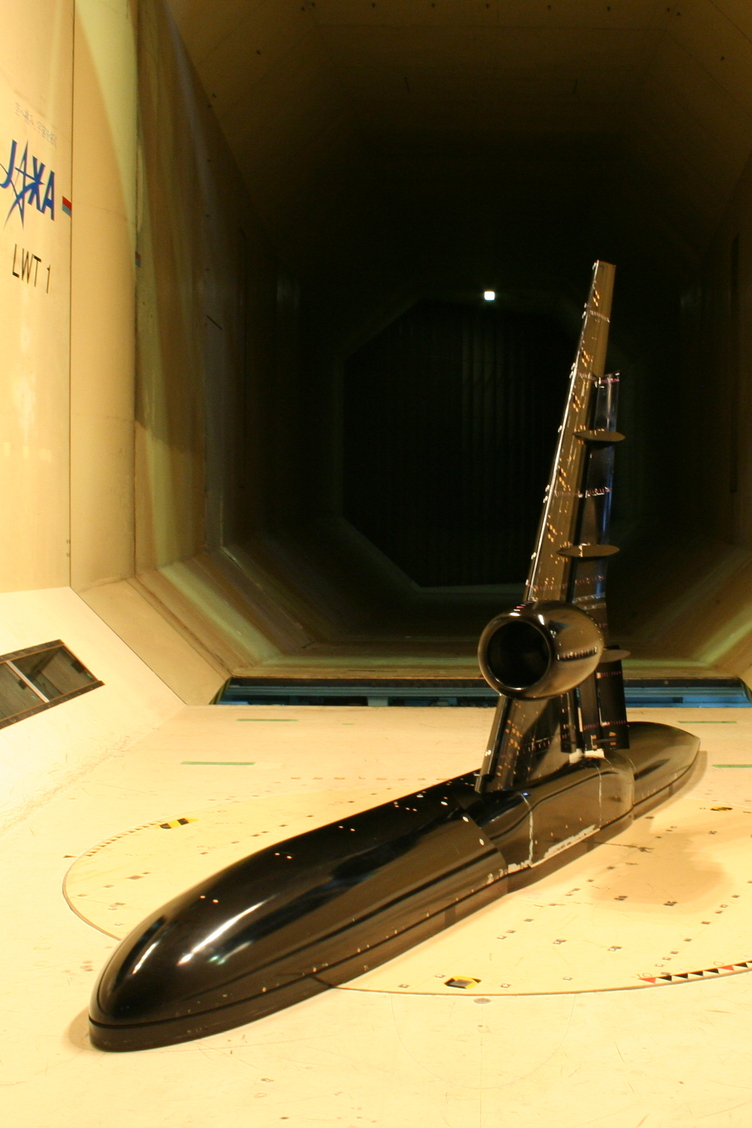
\includegraphics[width=0.5\columnwidth]{img/hlpw/jsm}
    \caption{A model of the JSM aeroplane in a wind tunnel.}
    \label{fig_hlpw_jsm}
\end{wrapfloat}
The main challenges in the simulation are the computation of drag and lift, with particular concern for the critical stall mechanism.
Lift generation tends to increase with increased angles of attack of a wing.
However, for a big enough angle of attack, the process abruptly interrupts and wings stop generating lift;
this phenomenon is called stall and should be avoided as it makes the aeroplane unable to fly, possibly with dramatic consequences.
For this reason, we had access to experimental results at a number of angle of attacks, from low values that are at no risk of stall to high values that exhibit stall.
The challenge is, of course, to simulate stall at the correct angle of attack.

The workshop proposed two configurations of the JSM for simulation, one with a nacelle (the \emph{pylon on} case) and one without a nacelle.
Given the small difference in reference aerodynamic forces given by experiments in the two cases, a difference of about \SI{2}{\percent}, we only focused on the \emph{pylon on} test case, which is the most complex and realistic of the two.

The organisers invited participants to test on two given meshes, a fine one to use as is and a coarser one to use with mesh adaptivity techniques.
Since the method we develop uses mesh adaptivity, we opted for the second approach, but we still generated our own mesh from the provided CAD files because the given mesh was not coarse enough.
It is worth pointing out at this point that our methodology can use a very coarse mesh as an initial mesh, the only requirement being that the geometric description of the surfaces, in this case of the aeroplane, be good enough to capture the geometric features.
The reason for this is that adaptive refinement near the surface does not improve the surface description in the sense that new points are not projected on the CAD shape from which the mesh was generated, as no CAD information is kept in the mesh.
Apart from this constraint, however, the volume mesh can be very coarse and the adaptive refinement will take care of adding mesh points where needed.
In particular, no specialised meshing knowledge is needed, nor any a priori knowledge of the features of the solution.

\section{Numerical tripping}
\label{sec_tripping}
The simulation of the stall cases was more challenging than the rest.
This is because stall is, from a physical point of view, generated by flow separation, in particular at the wing tip and near the wing-body junction, that detaches the flow and negatively affects the generation of lift.
The flow fields for the non-stalling configurations, which are well attached to the wing, are somewhat easier to reproduce; the transition to turbulence and consequent separation, on the other hand, were not.
We noted, in our first attempts, that the flow was not separating as expected.
Something similar happens with other numerical methods and the reason is that the inflow field, that is usually taken to be constant, is \emph{too perfect} to accurately represent reality.
In other words, no experiment in any wind tunnel will ever have a perfectly uniform and constant inflow, as is the case in numerical simulations, but rather an already chaotic inflow coming from air recirculation through the wind tunnel itself.
This means that the simulation would need a very long startup time to allow for numerical errors, the digital equivalent of physical perturbations, to grow and propagate in the flow field and reproduce a similar behaviour.

In the literature, an effective workaround is to add a small white-noise volume source term to the equation that has the effect of simulating this random perturbation in the inflow field.
In an attempt to strike a balance between a term that goes unnoticed and one that dominates over other effects, we scaled the white noise by \SI{5}{\percent} of the maximum of the pressure gradient.
We called this method \emph{numerical tripping} of the solution.

\section{Results overview}
\label{sec_results}
I will not go into the detailed results analysis for the test case, which is reported in the attached paper, but rather give an overview of the results and discuss their significance.

We performed simulations for a number of angles of attack in the range \((4, 23)\) starting from an initial mesh of just around \num{2.5e6} vertexes.
Unlike the experiment, which was performed on a half aeroplane profile, we created a mesh of a full profile to avoid modelling error introduced by a symmetry wall.
Figure~\ref{fig_hlpw_mesh} shows the surface mesh on the aeroplane geometry that we created, with Figure~\ref{fig_hlpw_meshDetail} showing the finest bits where the geometry is more complex.
\begin{figure}
  \centering
  \subfloat[][Surface mesh\label{fig_hlpw_meshAll}]
  {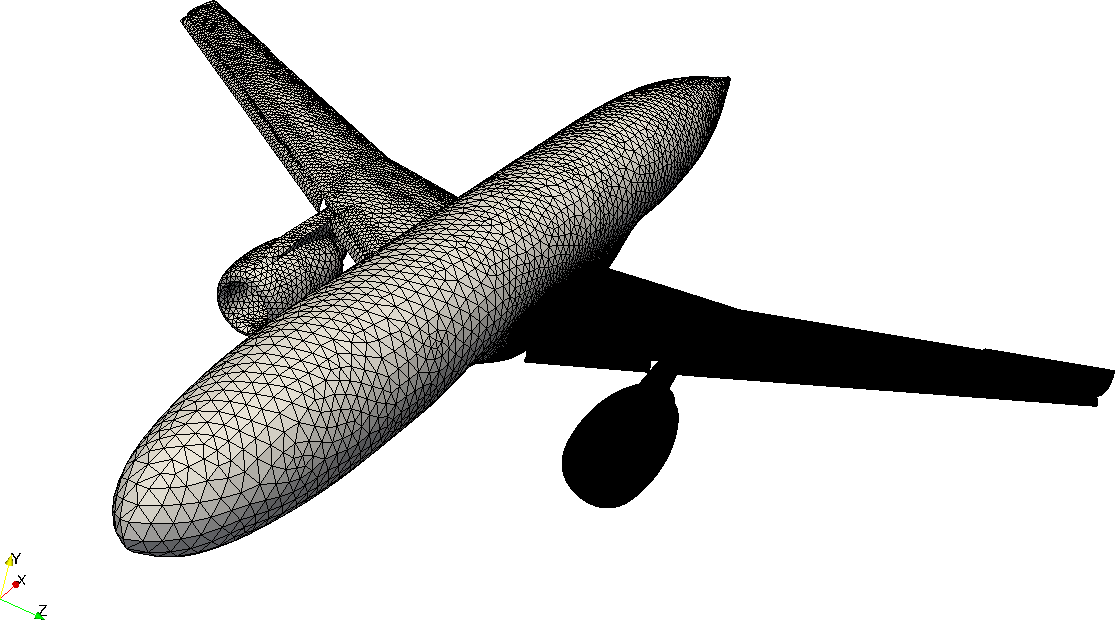
\includegraphics[width=0.45\textwidth]{img/hlpw/mesh}}
  \quad
  \subfloat[][Detail of wing mesh\label{fig_hlpw_meshDetail}]
  {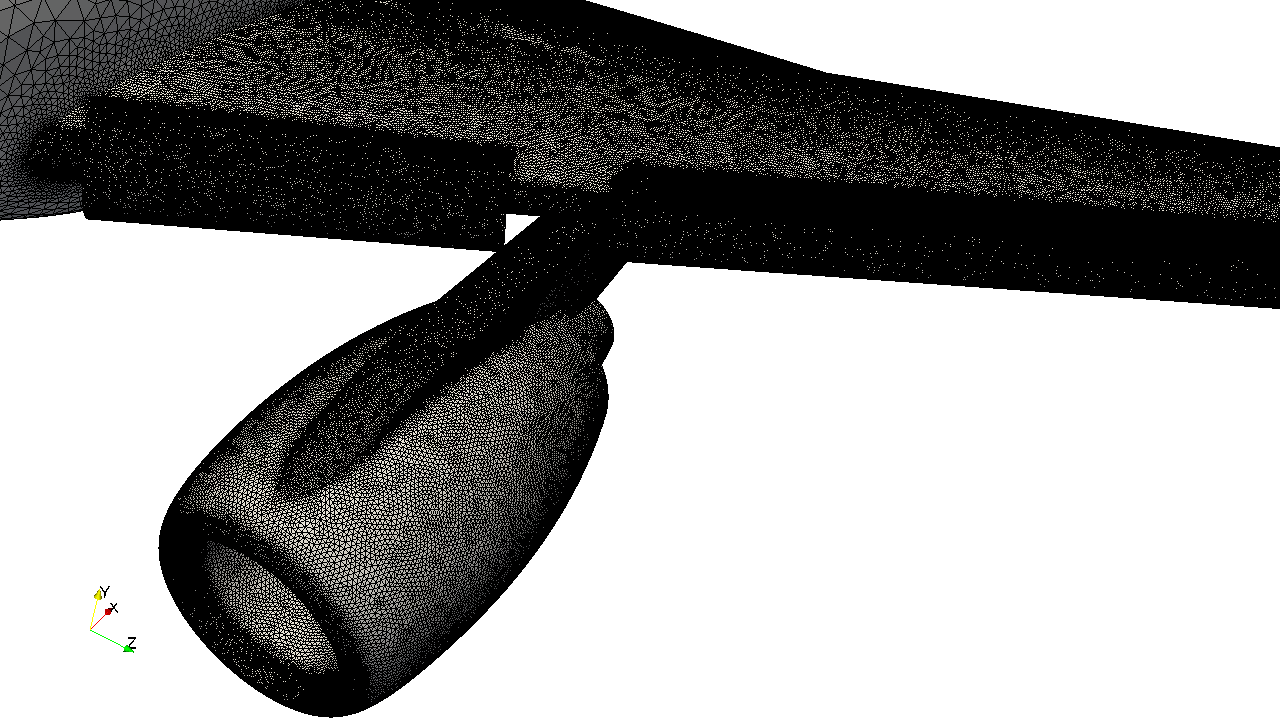
\includegraphics[width=0.45\textwidth]{img/hlpw/meshDetail}}
  \caption{The surface mesh we generated (left) and a detail of the mesh on the wing (right).}
  \label{fig_hlpw_mesh}
\end{figure}


Our starting mesh is significantly coarser than the provided one and allows for very cheap simulations.
At the end of our adaptive simulations, in which at each iteration we refined \SI{5}{\percent} of the cells, the finest meshes we had counted only \num{5e6} to \num{1e7} vertexes; for comparison, the tetrahedral mesh provided by the workshop had around \num{2.1e7} vertexes, meaning that even on our final runs we spent between a half and a fourth of the cost of running on the provided mesh.

We observed mesh convergence to experimental data for the lift coefficient within \SI{5}{\percent} for all the cases we ran, with a slightly bigger error of about \SI{10}{\percent} for the drag coefficient.
This is no surprise as the drag is notoriously more noisy and the typical drag signal oscillates noticeably, significantly more than the lift signal.

More importantly, for the configurations for which a stall is expected we were able to qualitatively simulate the stall mechanism, represented by a sharp drop in the lift force, for an angle of attack which differs from the experimental one by about \SI{1}{\degree}.

This is the most important feature of our results, and a remarkable achievement: our simulations were the only one to be time dependent, feature adaptivity and solve the full Navier-Stokes equations, and with the combination of these features we were able to both predict aerodynamic forces to values within experimental ranges and reproduce the correct physical separation in the flow field.
I would like to point out that nowhere in the code do we specify that we are interested in the separation, but we only ask for drag and lift.
The correct prediction of separation, together with the pressure profiles and other local quantities are simply a by-product of the method, that we were still able to recover without explicitly asking for them.

As an example, consider the visualisation in Figure~\ref{fig_hlpw_oil}, where experimental data from surface oil flow visualisation is compared to our simulation results.
\begin{figure}
  \centering
  \subfloat[][\(\alpha = 10.48^\circ\)\label{fig_hlpw_pylon_10_48_exp}]
  {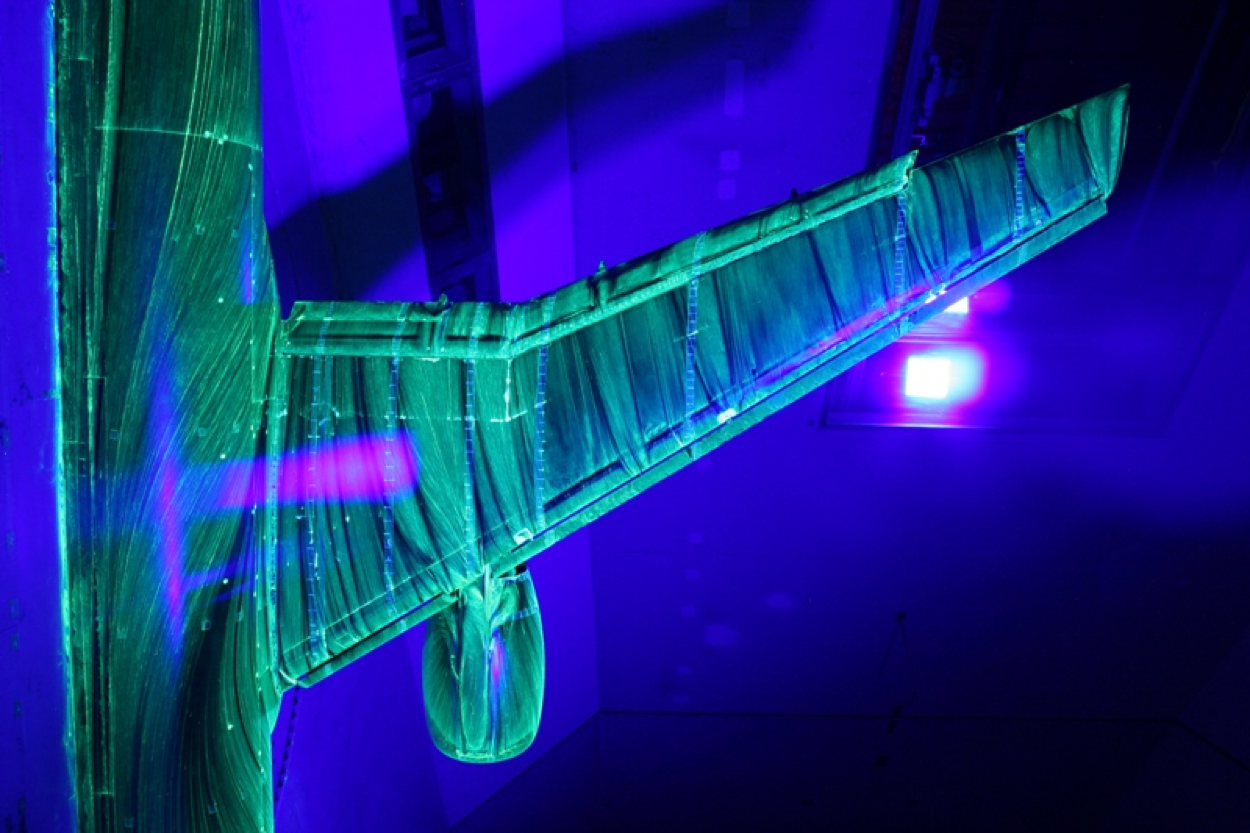
\includegraphics[width=0.45\textwidth]{img/hlpw/pylon_10_48_exp}}
  \quad
  \subfloat[][\(\alpha = 10.48^\circ\)\label{fig_hlpw_pylon_10_48_sim}]
  {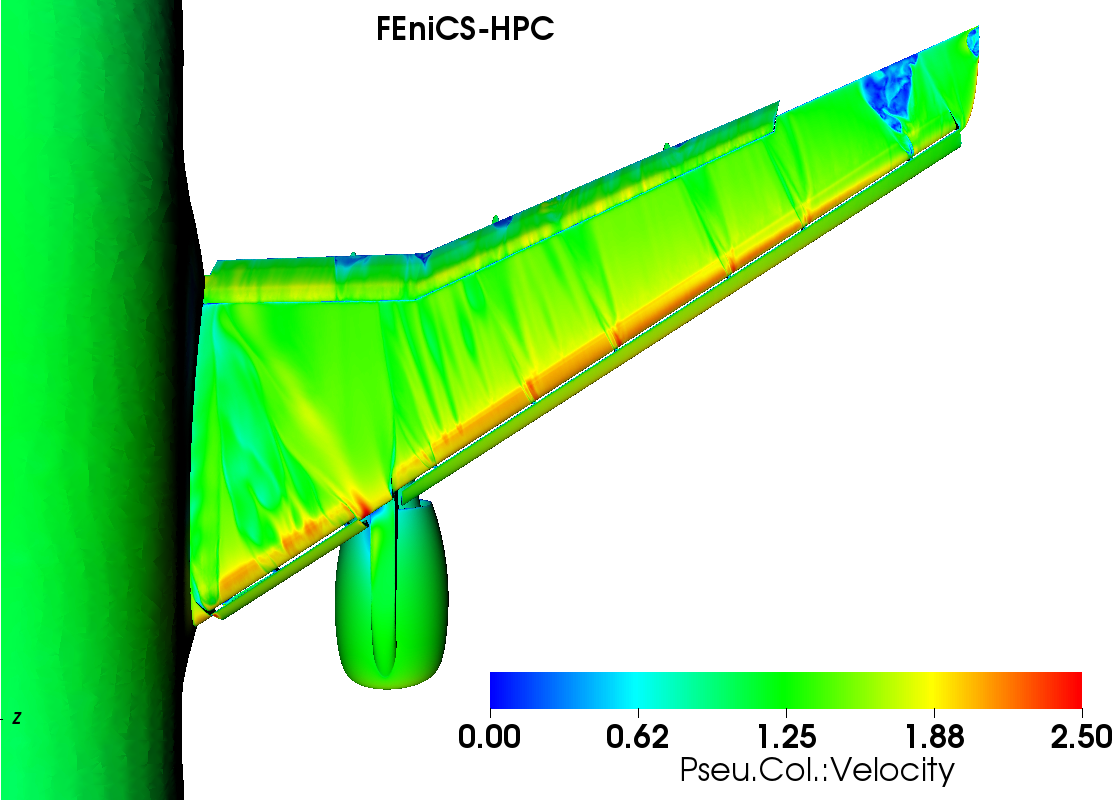
\includegraphics[width=0.45\textwidth]{img/hlpw/pylon_10_48_sim}}
  \\
  \subfloat[][\(\alpha = 18.58^\circ\)\label{fig_hlpw_pylon_18_58_exp}]
  {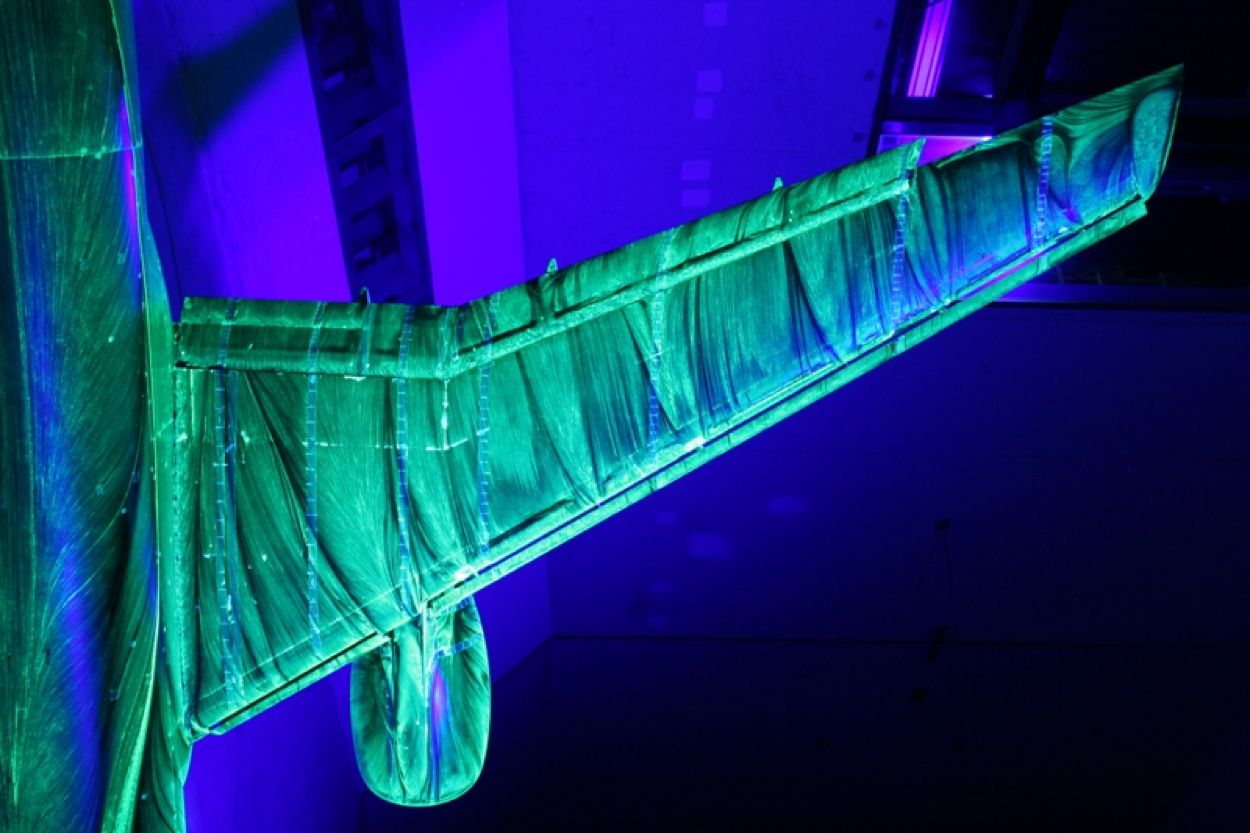
\includegraphics[width=0.45\textwidth]{img/hlpw/pylon_18_58_exp}}
  \quad
  \subfloat[][\(\alpha = 18.58^\circ\)\label{fig_hlpw_pylon_18_58_sim}]
  {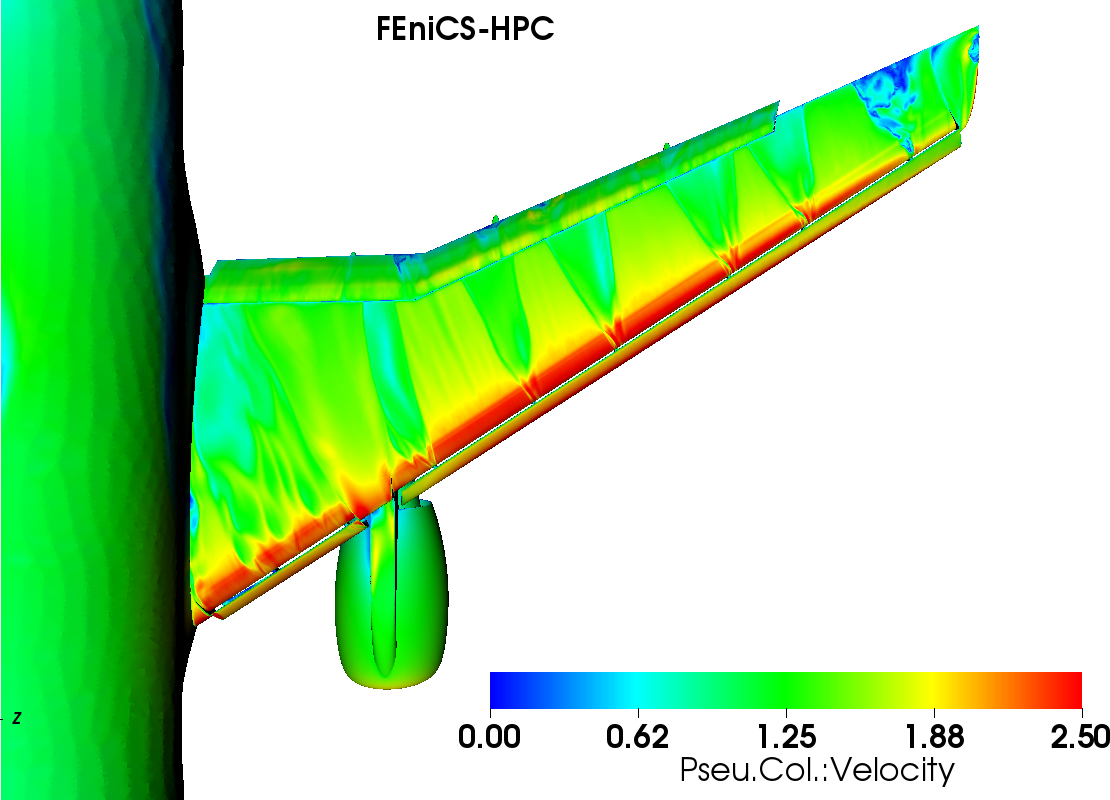
\includegraphics[width=0.45\textwidth]{img/hlpw/pylon_18_58_sim}}
  \\
  \subfloat[][\(\alpha = 21.57^\circ\)\label{fig_hlpw_pylon_21_57_exp}]
  {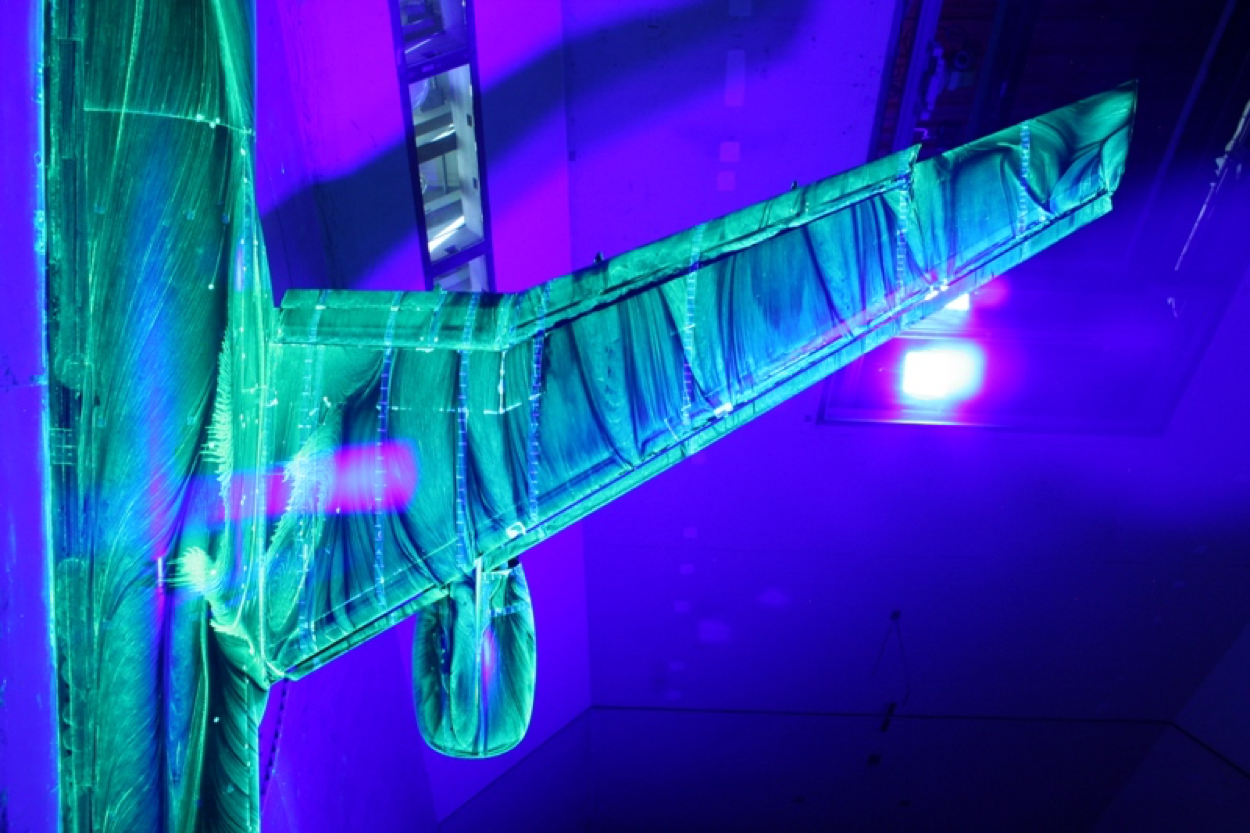
\includegraphics[width=0.45\textwidth]{img/hlpw/pylon_21_57_exp}}
  \quad
  \subfloat[][\(\alpha = 22.56^\circ\)\label{fig_hlpw_pylon_22_56_sim}]
  {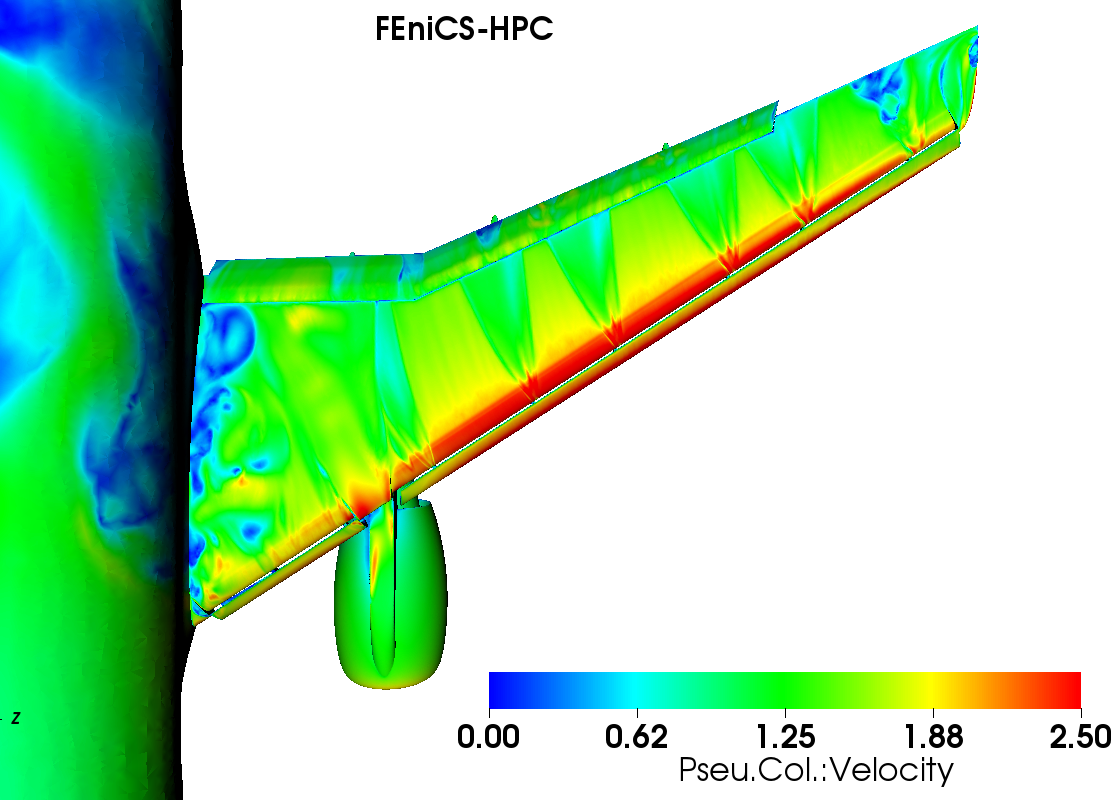
\includegraphics[width=0.45\textwidth]{img/hlpw/pylon_22_56_sim}}
  \\
  \caption{Comparison of surface oil flow visualisation from the wind tunnel and velocity profiles from our simulations.}
  \label{fig_hlpw_oil}
\end{figure}
What should be noticed in Figure~\ref{fig_hlpw_oil} is that the simulation results closely match the profiles in the experimental setup, in particular the V-shaped structures originating from where the leading edge of the wing is connected to the flaps.
In the first two rows the flow is attached as we are not at the stall angle yet, but the third row shows an important additional feature: separation at the wing-body junction, visually denoted by the blue, low velocity area on the left of Figure~\ref{fig_hlpw_pylon_22_56_sim}.

To give another point of view on the same phenomenon, Figure~\ref{fig_hlpw_pylon_22_56_vorticity} visualises the separation via the vorticity in the volume.\begin{figure}
  \centering
    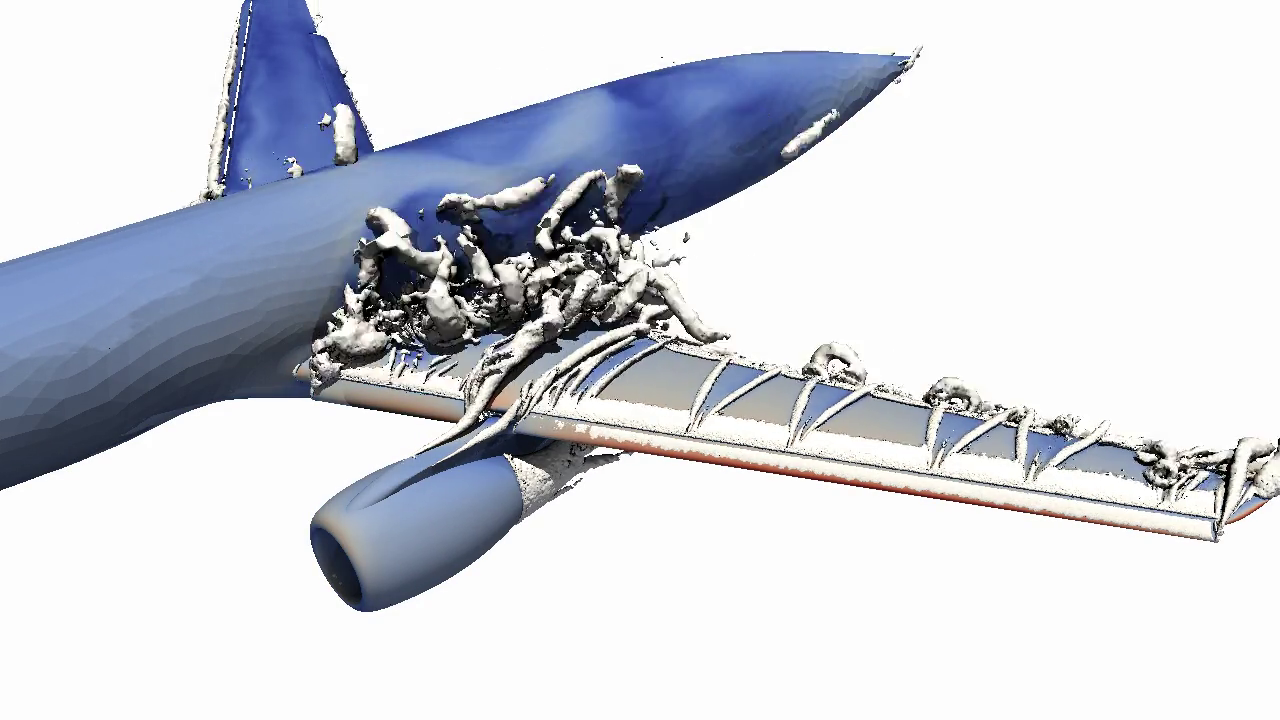
\includegraphics[width=\columnwidth]{img/hlpw/pylon_22_56_vorticity}
    \caption{Visualisation of turbulent separation via vorticity computed with the Q-criterion.}
    \label{fig_hlpw_pylon_22_56_vorticity}
\end{figure}
It represents a snapshot of a fully-developed flow field, showing how the turbulent separation grows from the wing-body junction

Again, I think it is worth pointing out that the code was not tuned to resolve the separation, but only the aerodynamic forces; the rest is a by-product of the method that naturally resolves the correct physical mechanisms at play, in this case stall.

  \chapter{High-performance computing in the cloud era}
\label{cha_hpcCloud}


  \chapter{Cardiac Radiofrequency Ablation}
\label{cha_rfa}
The rest of this thesis is devoted to a specific application to which I devoted a good share, if not the lion's share, of my time during my PhD: radiofrequency ablation.

\section{Radiofrequency ablation}
\label{sec_rfa}
Radiofrequency ablation is a minimally invasive treatment in which a catheter is used to deliver heat to a target tissue with the goal of burning it.
Heat is delivered by an electric current at a radio frequency of about \SI{500}{\kHz}, whence the name of the procedure, and is used to permanently damage the tissue of the patient in a very localised manner.
However counterproductive this might seem, it is not, and radiofrequency ablation is routinely used to treat a number of conditions such as hyperopia, asthma, gastric reflux, hepatic tumor, apnoea and, last but not least, cardiac arrhythmia.
The general idea of radiofrequency ablation is that causing controlled lesions in a tissue can be used to cure worse conditions, making it the lesser of two evils; some cardiac arrhythmias, for example, are caused by electric impulses propagating in the heart to areas where they should not, eliciting muscular contractions that affect the correct pace of the heart.
Burnt tissue, however, is known to be electrically insulating.
We can thus affect the electric circuit in a patient's heart, and in particular we can cut unwanted branches, by generating lesions that form a barrier that electricity cannot cross.

Not all treatments are equally safe, and the treatment of cardiac disorders is by far the most prone to risks and complications, even life-threatening: on average, around \SI{5}{\percent} of the administrations of cardiac radiofrequency ablation result in unexpected complications, a much higher rate than the other use cases mentioned above.

The risks with cardiac radiofrequency ablation, from now on \emph{RFA}, include the formation of cloths (or thrombi), when heat coagulates blood, and steam pop formation, arising when the temperature of the tissue is high enough that the water inside it evaporates.
Both scenarios are bad: thrombi have the potential to obstruct blood vessels if they accumulate in the circulatory system, but steam pops result in perforations of the cardiac wall.
When the perforation is transmural, meaning it pierces the heart from side to side, the patient's life is in great danger.
The pop is so violent it can literally be heard from outside the patient's body by the doctors in the room.
As a guideline, we consider that thrombi form in the blood when it reaches \SI{80}{\celsius}, while steam pop occur in the tissue at a temperature of \SI{100}{\celsius}; in contrast, tissue is considered irreversibly damaged at a temperature of \SI{50}{\celsius}.
The goal is then to bring a large enough portion of cardiac tissue to a temperature of \SI{50}{\celsius} while keeping the blood temperature below \SI{80}{\celsius} and the tissue temperature below \SI{100}{\celsius}.

RFA is administered to a patient that, although sedated, is still awake, and the doctor performing the procedure pushes the catheter through the patient's body, entering from the hip, manually applying pressure.
Several factors account for a less than ideal situation, most importantly the facts that the patient is not completely still -- his heart is beating -- and the doctor's pressure is not constant in time.
All these contribute to the high variability in the quality of the results of the procedure: although several different protocols are common, sometimes the lesions are too small, not blocking electricity properly and requiring a second administration, while sometimes too much power is delivered, resulting in complications.
On top of it, during the administration of the procedure it is hard to assess what is going on inside the patient, as inspecting the size of the lesion that is forming in the tissue is all but easy.
It is clear that this scenario can benefit from the help of numerical simulations to better understand what happens at the patient during the procedure, and this is the mission we set off to accomplish.

\section{Lesion assessment}
\label{sec_rfaLesion}
RFA is administered according to protocols.
A \emph{protocol} is a combination of values for pressure, power and time such as (\SI{20}{g}, \SI{30}{W}, \SI{10}{s}) meaning that the catheter should be held with a pressure of 20 grams, delivering 30 Watts of energy for 10 seconds\footnote{The use of the word \emph{pressure} to refer to a quantity in grams is typical for this application.}.

Manufacturers of medical devices use models, to some extent, to advise medical doctors on what protocols to use for a session of radiofrequency ablation.
These models are quite coarse-grained, often combining all three parameters in a protocol with some regression technique used a posteriori on experimental data from tests on animal tissue.
Although they are better than nothing, these models suffer from the limitations caused by condensing too much information in a single number and lack physical connection to the real scenario.
A mathematical model that draws from physical principles has the potential to do better.

\section{Mathematical modelling}
\label{sec_rfaModel}
In this section I will go through the modelling intervention that we performed to build a so-called \emph{digital twin} of the RFA procedure.

\subsection{Governing equations}
\label{sub_rfaEquations}
The RFA process is a multi-physics system involving fluid flow, current flux and thermal diffusion.

We used the incompressible Navier-Stokes equations to describe the fluid flow, which we already encountered in Equation~\eqref{eq_ns} in Section~\ref{sec_cfd} but that I report for convenience:
\begin{equation}
  \left\{
    \begin{aligned}
      &\partial_{t} \vec{u} (\vec{u} \cdot \grad) \vec{u} - \div\sigma(\vec{u},p) = \vec{0} \\
      &\div \vec{u} = 0
    \end{aligned}
  \right.
  \label{eq_rfaNS}
\end{equation}
where \(\vec{u}\) is the velocity, \(p\) is the pressure and \(\sigma(\vec{u},p) = 2 \nu \sym\grad \vec{u}\) is the stress tensor.

The electrical potential can be described as the solution to a Poisson-type equation.
This is a good approximation because the characteristic time in the evolution of radiofrequency currents is much shorter than that of the other phenomena considered in this simulation, so we can assume that the electrical potential is quasi-static and avoid solving the whole Maxwell equations in favour of a simpler elliptic equation.
We have
\begin{equation}
  \div(\sigma(T)\grad\Phi) = 0
  \label{eq_rfaPotential}
\end{equation}
where \(\Phi\) is the electrostatic potential and \(\sigma(T)\) is the electrical conductivity, that we consider as a function of the temperature \(T\).\footnote{It is an unfortunate coincidence that both the stress tensor and the electrical conductivity are denoted by the letter \(\sigma\) in the literature of the respective fields, but in this work they have different arity so no confusion should arise.}
This equation has to be solved with an additional constraint: during the RFA procedure, the machine used to provide power to the catheter does so trying to keep the dissipated power to a constant value \(P\) -- the one that appears in the protocol.
Recalling that, in electrostatics, the dissipated power is given by \(P = \vec{E} \cdot \vec{J}\) where the electrostatic field is \(\vec{E} = -\grad\Phi\) and the electrostatic current is \(\vec{J} = \sigma \vec{E}\), Equation~\eqref{eq_rfaPotential} needs to be complemented with the constraint
\begin{equation}
  \int \sigma(T) \norm*{\grad\Phi}^2 = P
  \label{eq_rfaPowerConstraint}
\end{equation}

Finally, for heat dissipation we used a modification of Penne's bioheat equation that describes tissue heating by both convection and power dissipation from radiofrequency currents.
The final form, that we have been using in the model, reads
\begin{equation}
  \rho c(T) \left( \partial_{t} T + \vec{u} \cdot \grad T\right) - \div(k(T) \grad T) = \sigma(T) \norm*{\grad \Phi}^2
  \label{eq_rfaBioheat}
\end{equation}
featuring the density \(\rho\), the specific heat \(c\), the thermal conductivity \(k\) and the temperature \(T\).
\(\Phi\) and \(\sigma\) are the same as in Equation~\eqref{eq_rfaPotential} while \(\vec{u}\) is taken from Equation~\eqref{eq_rfaNS}.

\subsection{Catheter geometry}
\label{sub_rfaGeometry}
For this model we have been using a geometry based on the in vitro experiment that we want to reproduce.
The geometrical description, however, introduces a few improvements over the state of the art in these kinds of simulations.

First of all, the catheter geometry is quite complex in itself.
The outside of the catheter is an adiabatic body that insulates it thermally and electrically.
At its tip, however, there is an electrode on which the machine applies a potential difference to drive electric current.
Inside the electrode tip there is a glass piece, called \emph{thermistor}, that has a high thermal capacity and is used to keep the electrode's temperature low, preventing it from overheating.
Finally, at its core there is a channel that is used to inject coolant in the heart; to make things more complex, the channel has small outlets that pass through the thermistor and the electrode, in the count of six for the model used in the experiment.
We report an overview of the catheter geometry in Figure~\ref{fig_rfa_catheter}.
\begin{wrapfloat}{figure}{O}{0pt}
  \centering
    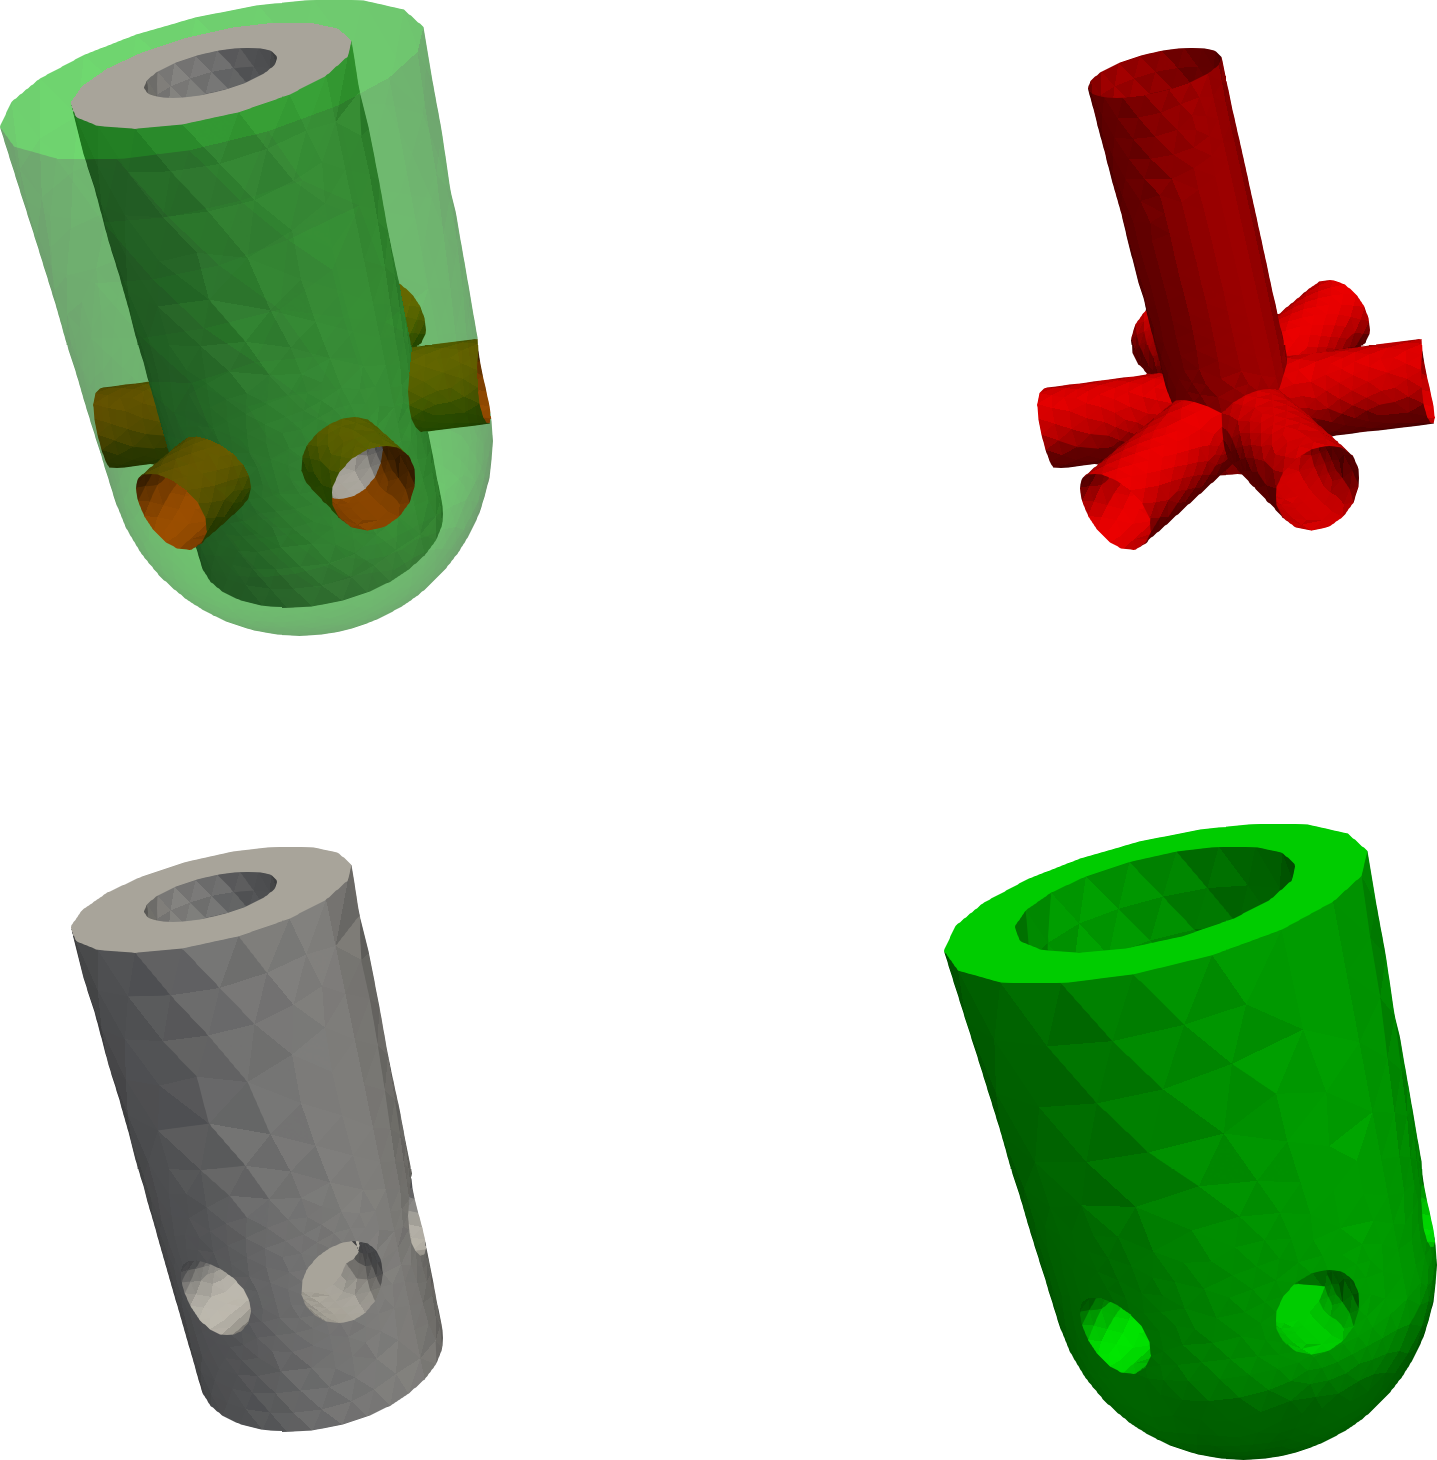
\includegraphics[width=0.5\columnwidth]{img/rfa/catheter}
    \caption{The components of the catheter tip: the inner channels in red, the thermistor in gray and the electrode in green.}
    \label{fig_rfa_catheter}
\end{wrapfloat}

Other works in the literature presented simulations of similar scenarios with a much simplified geometry: most in two spatial dimensions, with the ones in three dimensions having no description of the individual outlets of the inner channels, but instead a contiguous inlet surface going around the whole electrode.
An important improvement in our model, in particular in the geometrical description, was to use meshes of very accurate geometries that resolved all the details of the catheter.
We identify all the main parts of the catheter: the body, the electrode, the thermistor and the channels, with the electrode and the thermistor being part of the actual computational domain while the body and the inner channels are not but shape the boundary of the domain.

\subsection{External factors calibration}
\label{sub_rfaExternalFactors}
As far as the computational domain we used is concerned, it is composed by several additional parts.
The catheter is inserted in a part of the domain occupied by blood, with its tip, the electrode, touching another part, occupied by the tissue.
The tissue part is then resting on an additional part, which we call the \emph{external factors board}, or \emph{board} for short.
In the experiment, the tissue lied on a methacrylate board and the dispersive electrode, necessary for the ablation, was not placed in direct contact with the tissue but rather under this additional board.
The last part of the computational domain, then, corresponds to this additional object separating the tissue from the electrode.
I would like to point out that a similar situation happens in the administration of the real procedure where the dispersive electrode is placed on the patient, usually on the back, again rather far from the heart.

With the addition of this board, the computational domain looks like in Figure~\ref{fig_rfa_compDomain}, where we also reported its physical dimensions in meters for comparison.
\begin{wrapfloat}{figure}{O}{0pt}
  \centering
    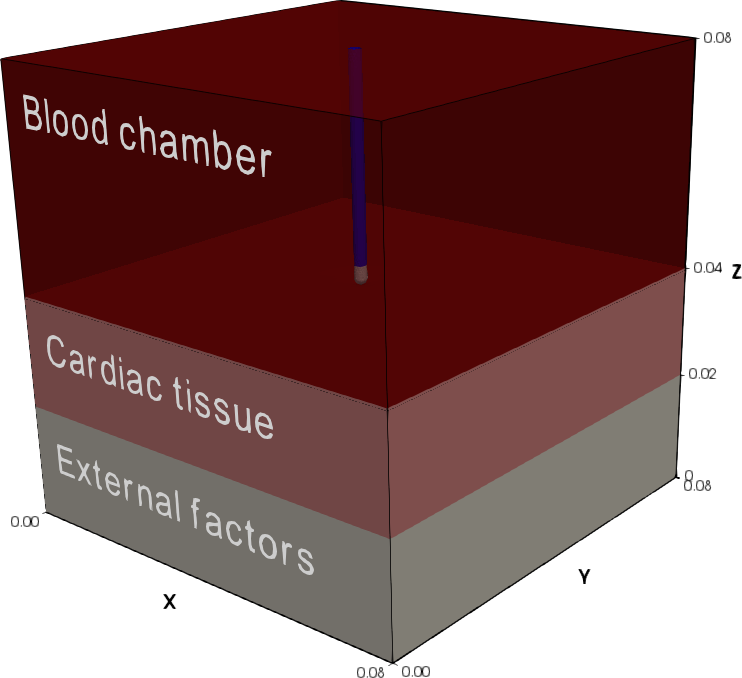
\includegraphics[width=0.5\columnwidth]{img/rfa/compDomain}
    \caption{The computational domain used for our simulations, consisting of the catheter in the blood chamber, with its tip touching the cardiac tissue, which is resting on the external factors board. Dimensions in meters.}
    \label{fig_rfa_compDomain}
\end{wrapfloat}

The presence of the external factors board also gives us the opportunity to calibrate the model to match the setup of the actual experiment, and this is where it gets its name from.
The domain we used in our simulations is much smaller than the actual domain used for the experiments.
This poses a problem as some of the electric power is dissipated outside the small volume we simulate, but it is difficult to keep track of it.
Luckily, we know from the RFA machine how much resistance the whole setup offers to it, so we can tune the \(\sigma\) of the board in order to match the same value.
This gives us a single parameter to tune the computational domain to simulate a much bigger volume; furthermore, the tuning is done only at the beginning of the simulation and then kept throughout the whole run.
I wish to note that the constraint of matching the system's impedance is very important because it ensures that the correct amount of power is distributed to the various components of the domain -- the blood, the tissue, etcetera -- so much so that in a previous work the same goal was achieved by changing the electrical impedance of the cardiac tissue.
Our solution is more elegant and does not affect the physical properties of the parts of the system we are more interested into; we therefore consider it a significant improvement over the state of the art.

\subsection{Elastic contact}
\label{sub_rfaElastic}
The tip of the electrode is in direct contact with the tissue.
During our investigation of the numerical simulation of RFA, it became clear how the geometry of this contact is of the utmost importance for an accurate simulation of the ablation procedure.
The reason is that the part of the electrode surface that is in contact with the tissue will provide electric current directly to it, while the part that is in contact with the blood will dissipate energy into the blood.
Electrons on the electrode, on which they can move freely as it is a good conductor, are in fact faced with the choice of flowing either in the blood or in the tissue.
We know from the theory of electromagnetism that electrons will flow into a medium in an amount directly proportional to the cross-sectional area of the medium and inversely proportional to its impedance; in other words, electrons will favour a medium that they can access through a large area and offers small resistance.
The setting can be modelled as an electric circuit in which current can flow in two parallel branches, one containing a resistance representing the tissue, the other containing a resistance representing the blood and the tissue in a sequence.
As detailed in the paper, we use this description to find that the power dissipated in the tissue is proportional to
\begin{equation}
  \alpha := \frac{A_{tissue}\sigma_{tissue}}{A_{blood}\sigma_{blood} + A_{tissue}\sigma_{tissue}}
  \label{eq_rfaPowerDistribution}
\end{equation}
It is clear that, to correctly reproduce a cardiac ablation, it is essential to know how much of the electrode is in contact with the tissue and how much with the blood; in other words, we need to know the geometry of the electrode-tissue contact, or our simulation, even with all the correct values for the various physical parameters, will behave differently from reality.
It is important to highlight that the electrode-tissue contact surface depends on the applied pressure which is specified in the RFA protocol.

We introduced a model of elastic contact to take this fact into account.
We modelled the configuration as an indentation problem of a rigid sphere -- the catheter tip -- into a half-space -- the cardiac tissue.
We chose to use an elastic material description for the tissue as this gives us the opportunity to use realistic values for the Young modulus and the Poisson ratio that are known in the literature, and also because it is a reasonable choice.
We borrowed knowledge from contact mechanics and described our indentation problem via an \emph{axisymmetric Boussinesq formulation}, which gives us the profile of the tissue surface for a given applied force. 
\begin{figure}
  \centering
    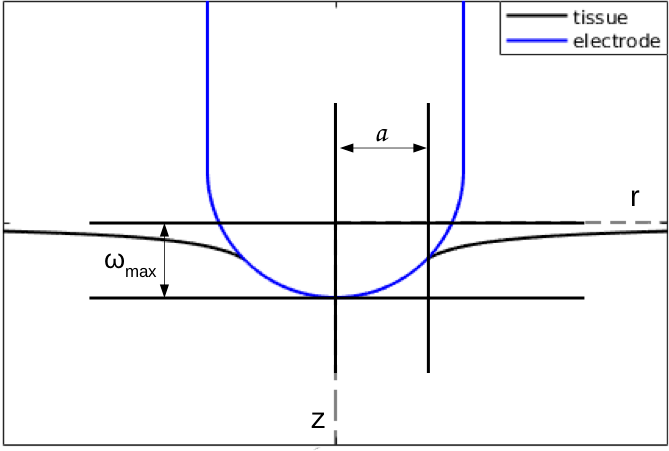
\includegraphics[width=0.75\columnwidth]{img/rfa/crossSectionContact}
    \caption{Sketch of the elastic contact profile: the tissue surface deforms to follow the indenting sphere.}
    \label{fig_rfa_crossSectionContact}
\end{figure}
Prior to the use of contact mechanics to compute a contact profile, numerical models of RFA simply considered a sharp insertion of the catheter into the tissue, meaning that the penetration depth of the catheter into the tissue was adjusted based on the exerted force, but the tissue surface was left unchanged (flat).
This led to an intrinsic overestimation of the electrode-tissue surface contact area that jeopardised the physics of the whole system.
A visual comparison of the two methods will make the difference clear: Figure~\ref{fig_rfa_tissueComparison} presents such comparison.
\begin{figure}
  \centering
    \subfloat[][\SI{10}{g} sharp.\label{fig_rfa_tissueSharp10g}]
    {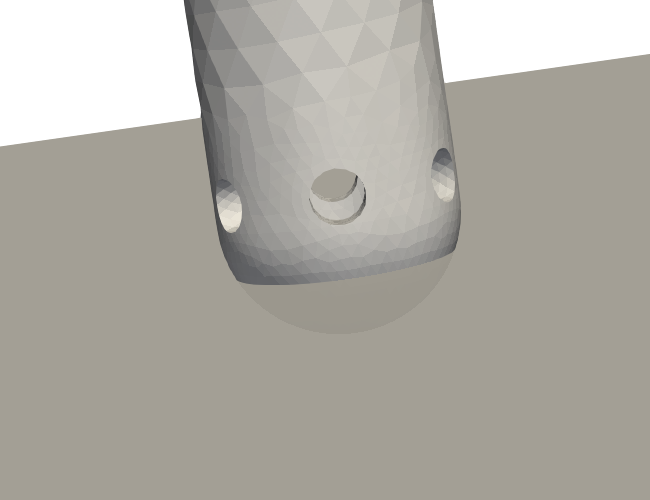
\includegraphics[width=0.3\textwidth]{img/rfa/tissueSharp10g}}
    \quad
    \subfloat[][\SI{20}{g} sharp.\label{fig_rfa_tissueSharp20g}]
    {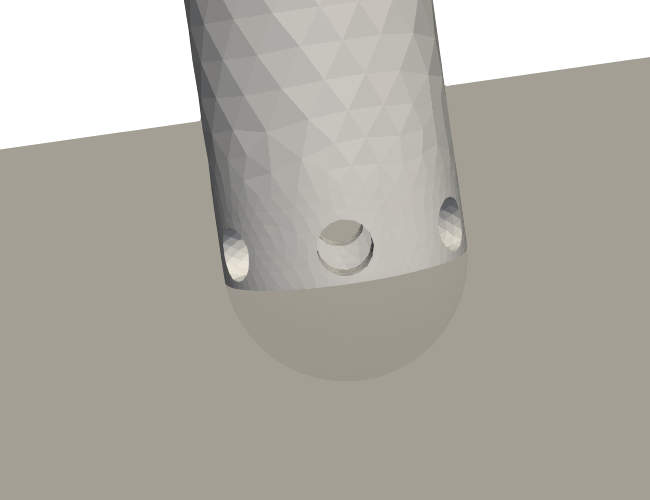
\includegraphics[width=0.3\textwidth]{img/rfa/tissueSharp20g}}
    \quad
    \subfloat[][\SI{40}{g} sharp.\label{fig_rfa_tissueSharp40g}]
    {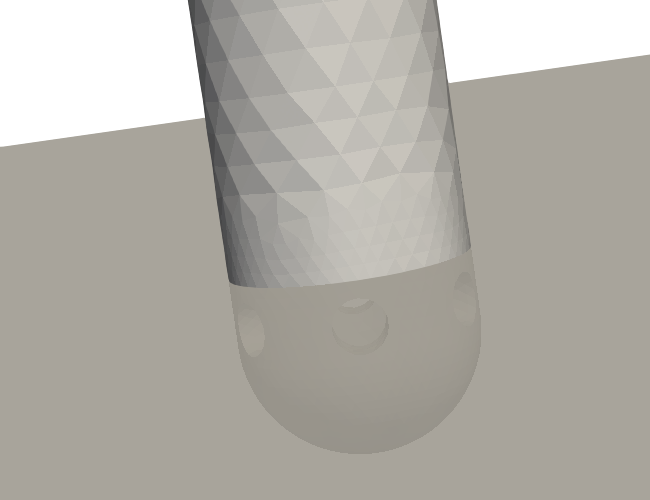
\includegraphics[width=0.3\textwidth]{img/rfa/tissueSharp40g}}
    \\
    \subfloat[][\SI{10}{g} elastic.\label{fig_rfa_tissueElastic10g}]
    {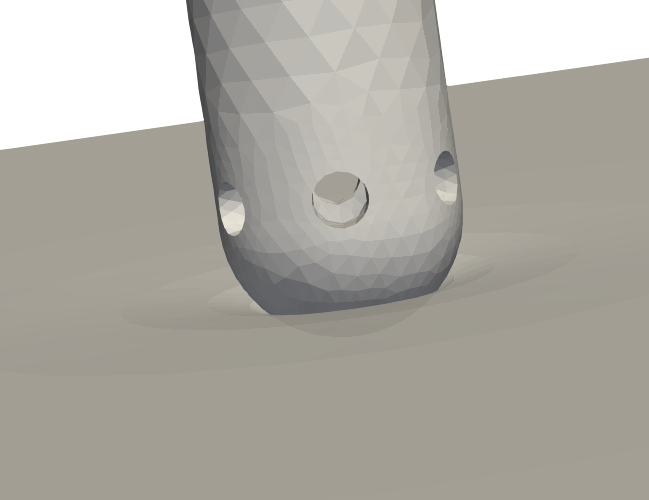
\includegraphics[width=0.3\textwidth]{img/rfa/tissueElastic10g}}
    \quad
    \subfloat[][\SI{20}{g} elastic.\label{fig_rfa_tissueElastic20g}]
    {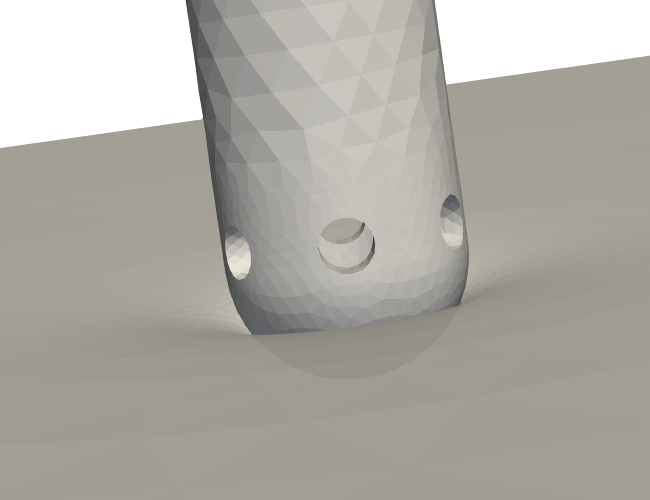
\includegraphics[width=0.3\textwidth]{img/rfa/tissueElastic20g}}
    \quad
    \subfloat[][\SI{40}{g} elastic.\label{fig_rfa_tissueElastic40g}]
    {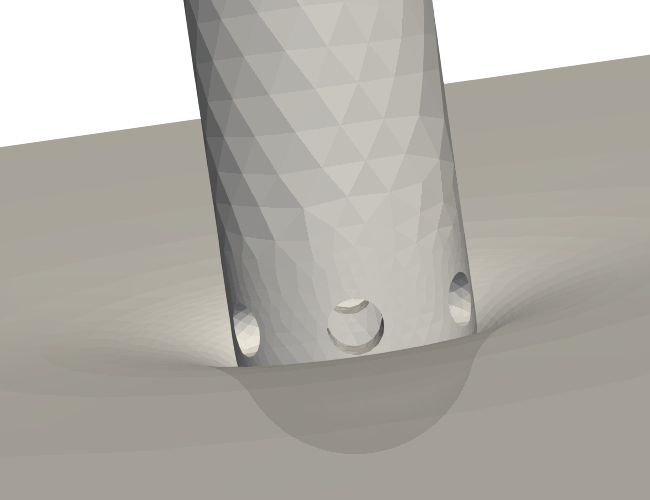
\includegraphics[width=0.3\textwidth]{img/rfa/tissueElastic40g}}
    \caption{Comparison of tissue-catheter contacts for sharp (top row) and elastic (bottom row) contact deformation models for three common values of pressure.}
    \label{fig_rfa_tissueComparison}
\end{figure}
The above discussion should now make sense: it immediately strikes the eye how one of the two approaches, the one represented in the bottom row of pictures, is more realistic.
If the difference is not dramatic in the \SI{10}{g} case, it is in the other two, especially in the \SI{40}{g} case where the displacement is such that the irrigation holes end up under the tissue surface, a clearly unphysical scenario.
The elastic deformation model that we introduced gives a much more realistic approximation of the electrode-tissue contact, resulting in a correct distribution of the electric current between the blood and the tissue.

I want to stress that the misbehavior caused by a computational mesh with an incorrect electrode-tissue contact is not caused by a parameter that can be tuned in the code, because it is a property of the shape of the solution to Equation~\eqref{eq_rfaPotential}.
Although one can still, despite an incorrect geometry, manage to deliver the correct amount of power to the tissue, this will affect the results of the simulation in the rest of the domain, for example in the blood, and ultimately deteriorate the physical accuracy of the simulation in a way that cannot be corrected.

Adding our elastic contact model was a crucial step toward a successful model and was very effective, while it also helped us better understand the physics of the radiofrequency ablation problem.


\subsection{Model summary}
\label{sub_rfaSummary}
Our model is ruled by Equations~\eqref{eq_rfaNS}, \eqref{eq_rfaPotential} and \eqref{eq_rfaBioheat} on a mesh generated according to the discussion in the preceding subsections.
These equations are equipped with a variety of boundary conditions: Figure~\ref{fig_rfa_bcs} shows a schematic representation of the domain, a detail of the catheter tip and all boundary conditions that differ from no-slip (\(\vec{u} = \vec{0}\)), zero current flux (\(\sigma(T)\grad\Phi \cdot \vec{n} = 0\)) and body temperature (\(T = T_b\)).
\begin{figure}
  \centering
    \def\svgwidth{\columnwidth}
    \input{img/rfa/bcs.pdf_tex}
    \caption{Schematic representation of our geometry and boundary conditions that differ from no-slip (\(\vec{u} = \vec{0}\)), zero current flux (\(\sigma(T)\grad\Phi \cdot \vec{n} = 0\)) and body temperature (\(T = T_b\)). On the right, a detail of the catheter's tip in front and top view.}
    \label{fig_rfa_bcs}
\end{figure}
In this figure, \(\vec{u}_{in}\) is the blood's inflow velocity, \(V_0\) is the applied potential, \(\vec{u}_s\) is the saline's inflow velocity and \(T_s\) is its temperature.

The choice of zero current flux on the boundaries of the domain is motivated by the need to make all the current flow to the dispersive electrode, which is what happens in reality.
However, the real domain is much bigger than the computational one from which some current should leave, so an even better approach would be to try and estimate the current that leaves our small domain and impose that flux on the boundary instead.

\section{Experimental setup and data}
\label{sec_experiment}
A good model is not very incisive if it does not match experimental data, which in the case of clinical procedures is often scarce.
In the case of RFA, luckily, we had access to an experimental facility where we performed test ablations in order to collect data.
These tests were not performed on humans, but rather on porcine cardiac tissue; this only affects the values of some physical parameters that we input to the code, but not the general idea and validity of our model.
The experimental setup consists of the catheter and the cardiac tissue, which is resting on a plastic slab.
This setup is submerged into a blood bath, which in turn is contained in a thermal reservoir.
A blood pump circulates the blood to simulate the flow of blood typical of a living patient, which is the main means of thermal dissipation.
The setup is pictured in Figure~\ref{fig_rfa_experiment}.
\begin{figure}
  \centering
    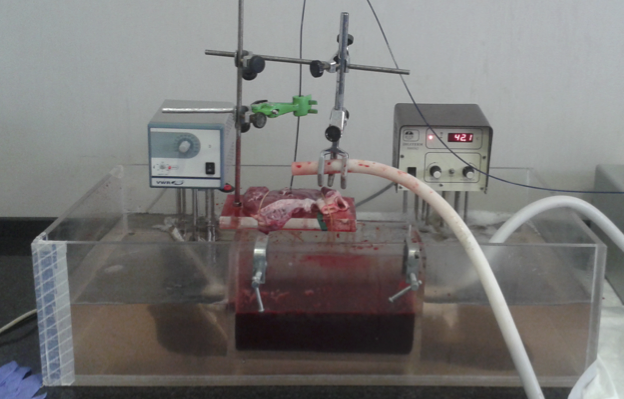
\includegraphics[width=\columnwidth]{img/rfa/experiment}
    \caption{The experimental setup that we aim to reproduce with our model: the tissue and the electrode are submerged in a blood bath where blood flows thanks to a pump.}
    \label{fig_rfa_experiment}
\end{figure}

With this setup, clinicians perform a radiofrequency ablation according to a given protocol on the tissue.
They later cut the tissue open where the ablation was performed and wash it with a special solution that reacts with burnt tissue, making it white.
This makes it possible to have a visual feedback of the lesion that the procedure caused.
Figure~\ref{fig_rfa_lesionExp} shows one such lesion, from the very same set of experiments.
For comparison, Figure~\ref{fig_rfa_lesionSim} shows a similar lesion as a result of a simulation using the model we developed.
\begin{figure}
  \centering
    \subfloat[][Experimental lesion.\label{fig_rfa_lesionExp}]
    {\includegraphics[width=0.45\textwidth]{img/rfa/lesionExp}}
    \quad
    \subfloat[][Simulated lesion.\label{fig_rfa_lesionSim}]
    {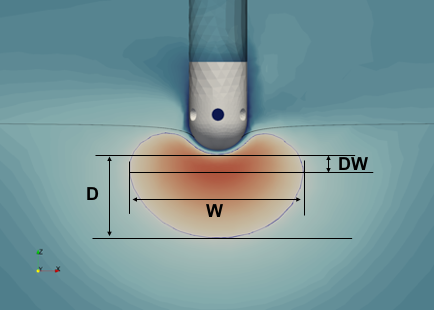
\includegraphics[width=0.45\textwidth]{img/rfa/lesionSim}}
    \caption{A lesion caused to real tissue in an experiment and a simulated lesion obtained with our code. On both figures we defined the quantities of interest that we used to validate our model against the available experimental data.}
    \label{fig_rfa_lesions}
\end{figure}
In Figure~\ref{fig_rfa_lesions} we highlighted the definitions of some quantities of interest that describe a lesion's shape, namely its width (W), its depth (D) and the depth of its maximum width (DW).
These quantities are very meaningful as they can be used to plan an administration of the procedure, and they are easy to compute both in vitro and in silico.
We validated our code and model against this data; all the details are in the attached paper but a brief overview of the results is in Section~\ref{sec_rfaResults}.

\section{Results overview}
\label{sec_rfaResults}
This section contains sample results from simulations of the model introduced in Section~\ref{sec_rfaModel}.
I do not want to delve into the details of data validation in favor of a more qualitative presentation: a quantitative discussion is deferred to the attached paper; here, it is enough to anticipate that we were able to validate the experimental data to a satisfactory level of accuracy.

Instead, I would like to show a typical visualisation of a simulation result.
Figure~\ref{fig_rfa_sim} shows two lesions simulated with protocols that differ in the applied pressure.
\begin{figure}
  \centering
    \subfloat[][\SI{10}{g}\label{fig_rfa_sim10g}]
    {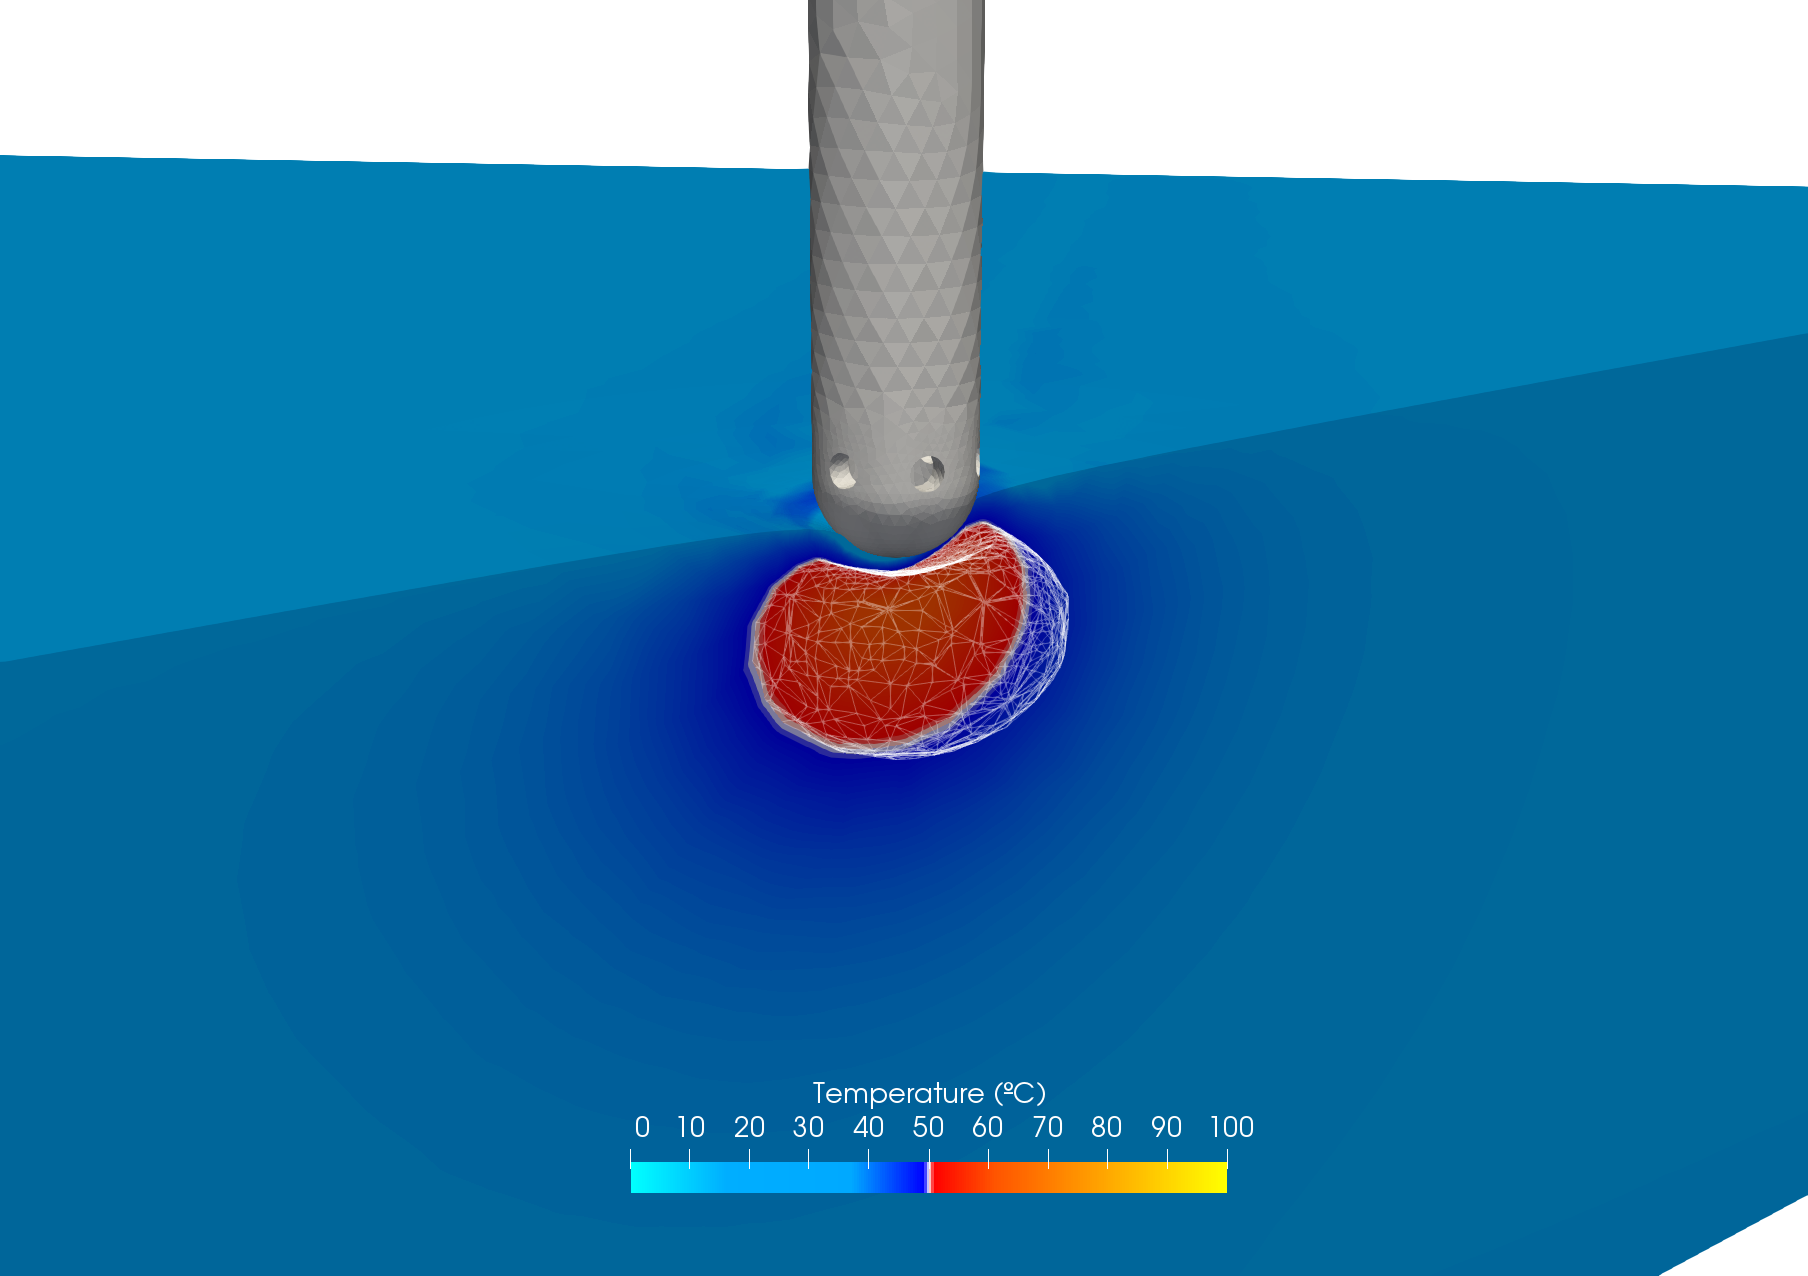
\includegraphics[width=0.45\textwidth]{img/rfa/elastic10g}}
    \quad
    \subfloat[][\SI{40}{g}\label{fig_rfa_sim40g}]
    {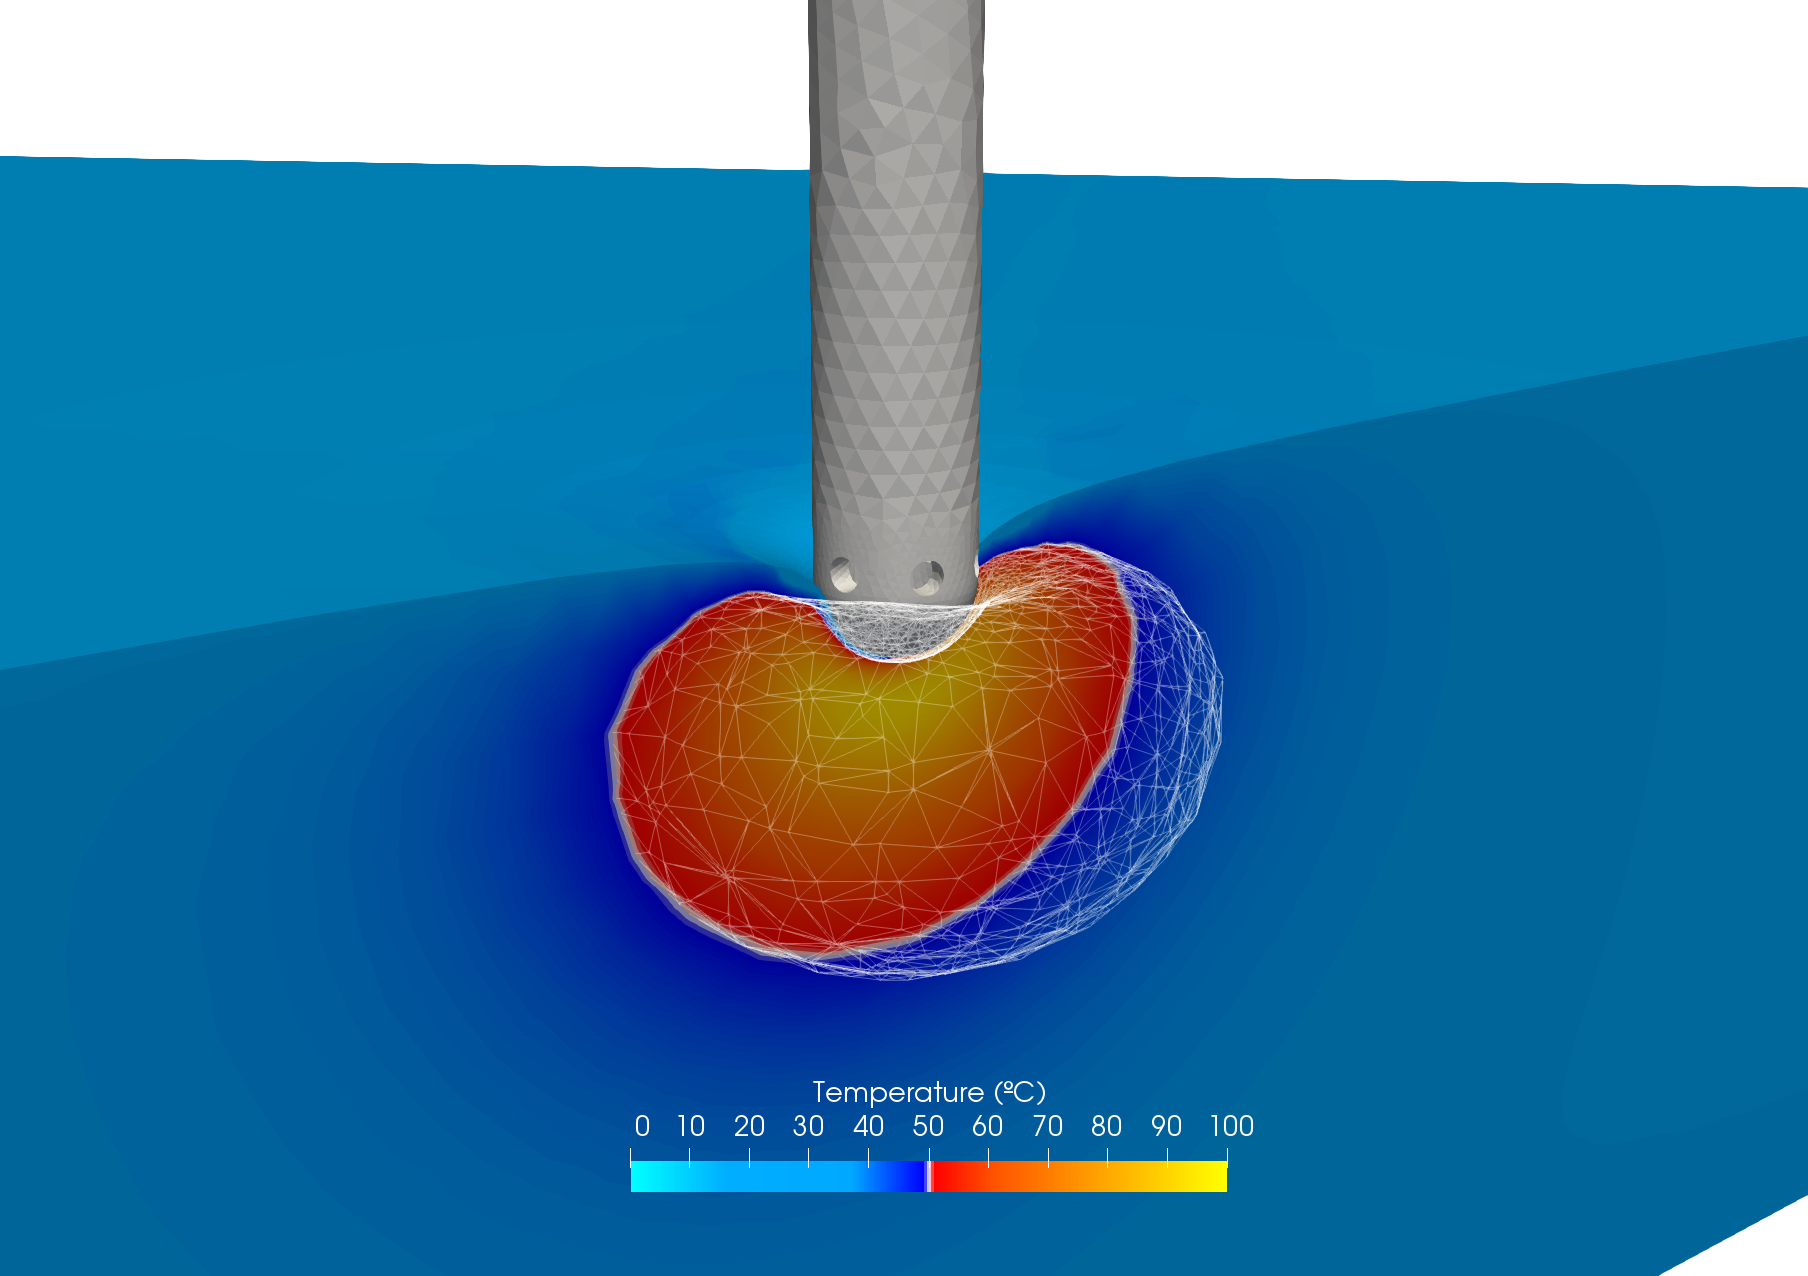
\includegraphics[width=0.45\textwidth]{img/rfa/elastic40g}}
    \caption{Simulated lesions for two protocols at \SI{10}{g} (left) and \SI{40}{g} (right). The view shows a cut through the cardiac tissue and an isosurface at \SI{50}{\celsius} that represents the lesion.}
    \label{fig_rfa_sim}
\end{figure}
The lesions are identified by the white isosurface, while the simulation also gives an estimate of the temperature reached inside the lesion, which is critical as we discussed in Section~\ref{sec_rfa}.
The results are consistent with our expectations: the lesion in Figure~\ref{fig_rfa_sim40g} is much bigger than that in Figure~\ref{fig_rfa_sim10g}, a consequence of the fact that the electrode-tissue contact area is bigger.
Datasets like those behind Figure~\ref{fig_rfa_sim} contain much more information than the various indexes used to estimate the lesion size that I mentioned in Section~\ref{sec_rfaLesion}, making them much more useful for clinical decision-making.
With detailed information on the size of the lesion it is possible to optimally plan the administration of the procedure to reduce the risk for the patient and improve the result.

\section[Future developments]{Cylindrical catheters, high and low flows, high-power ablation and beyond}
\label{sec_future}
Availability of experimental data is often low in medical applications, making it harder to test new protocols or techniques.
A reliable model makes the task easier as it allows to experiment at will in the digital twin with confidence that the behaviour is representative of the actual phenomenon.
For this reason, the model we built can be, and has been, used to test the effects of variations in the geometry, in the parameters, in the protocol, etcetera.
In this section I would like to point out possible present and future research directions that we can follow using the technology we developed.
\begin{itemize}
  \item \textbf{Cylindrical catheters.} The catheters we simulated when testing the model all have a spherical tip, in order to match the one used in the experiments we tried to reproduce. However, cylindrical tips are also common and one might ask if one of is better than the other. Cylindrical tips are flat and their electrode-tissue contact area changes much less with a perturbation in the applied pressure than the one of spherical catheters. Knowing how important the electrode-tissue surface area is, one might argue that cylindrical tips offer more stability in the results being less sensitive to variations in the applied pressure, that are systemic and difficult to eliminate completely. Since simulating a cylindrical tip is very easy with out model, as we only need to provide the code with a corresponding mesh, we can easily investigate this question.
  \item \textbf{High flow and low flow.} The blood flow in the heart during the ablation is the main means of thermal diffusion that, alongside the coolant injected by the catheter, helps to control the temperature rise. In our simulation we mainly used a fixed value for the inlet of the blood flow, a reasonable value that matched the experimental setup. In the human heart, however, the blood velocity varies noticeably from atria to ventricles, and in sedated patients it is likely smaller than in a regular heart. Figure~\ref{fig_rfa_saline} shows how the convection of the saline coolant is affected by the blood flow we routinely used (that we call \emph{high flow}, Figure~\ref{fig_rfa_salineHighFlow}) and by a weaker one (which we refer to as \emph{low flow}, Figure~\ref{fig_rfa_salineLowFlow}).
    \begin{figure}
      \centering
      \subfloat[][High flow\label{fig_rfa_salineHighFlow}]
      {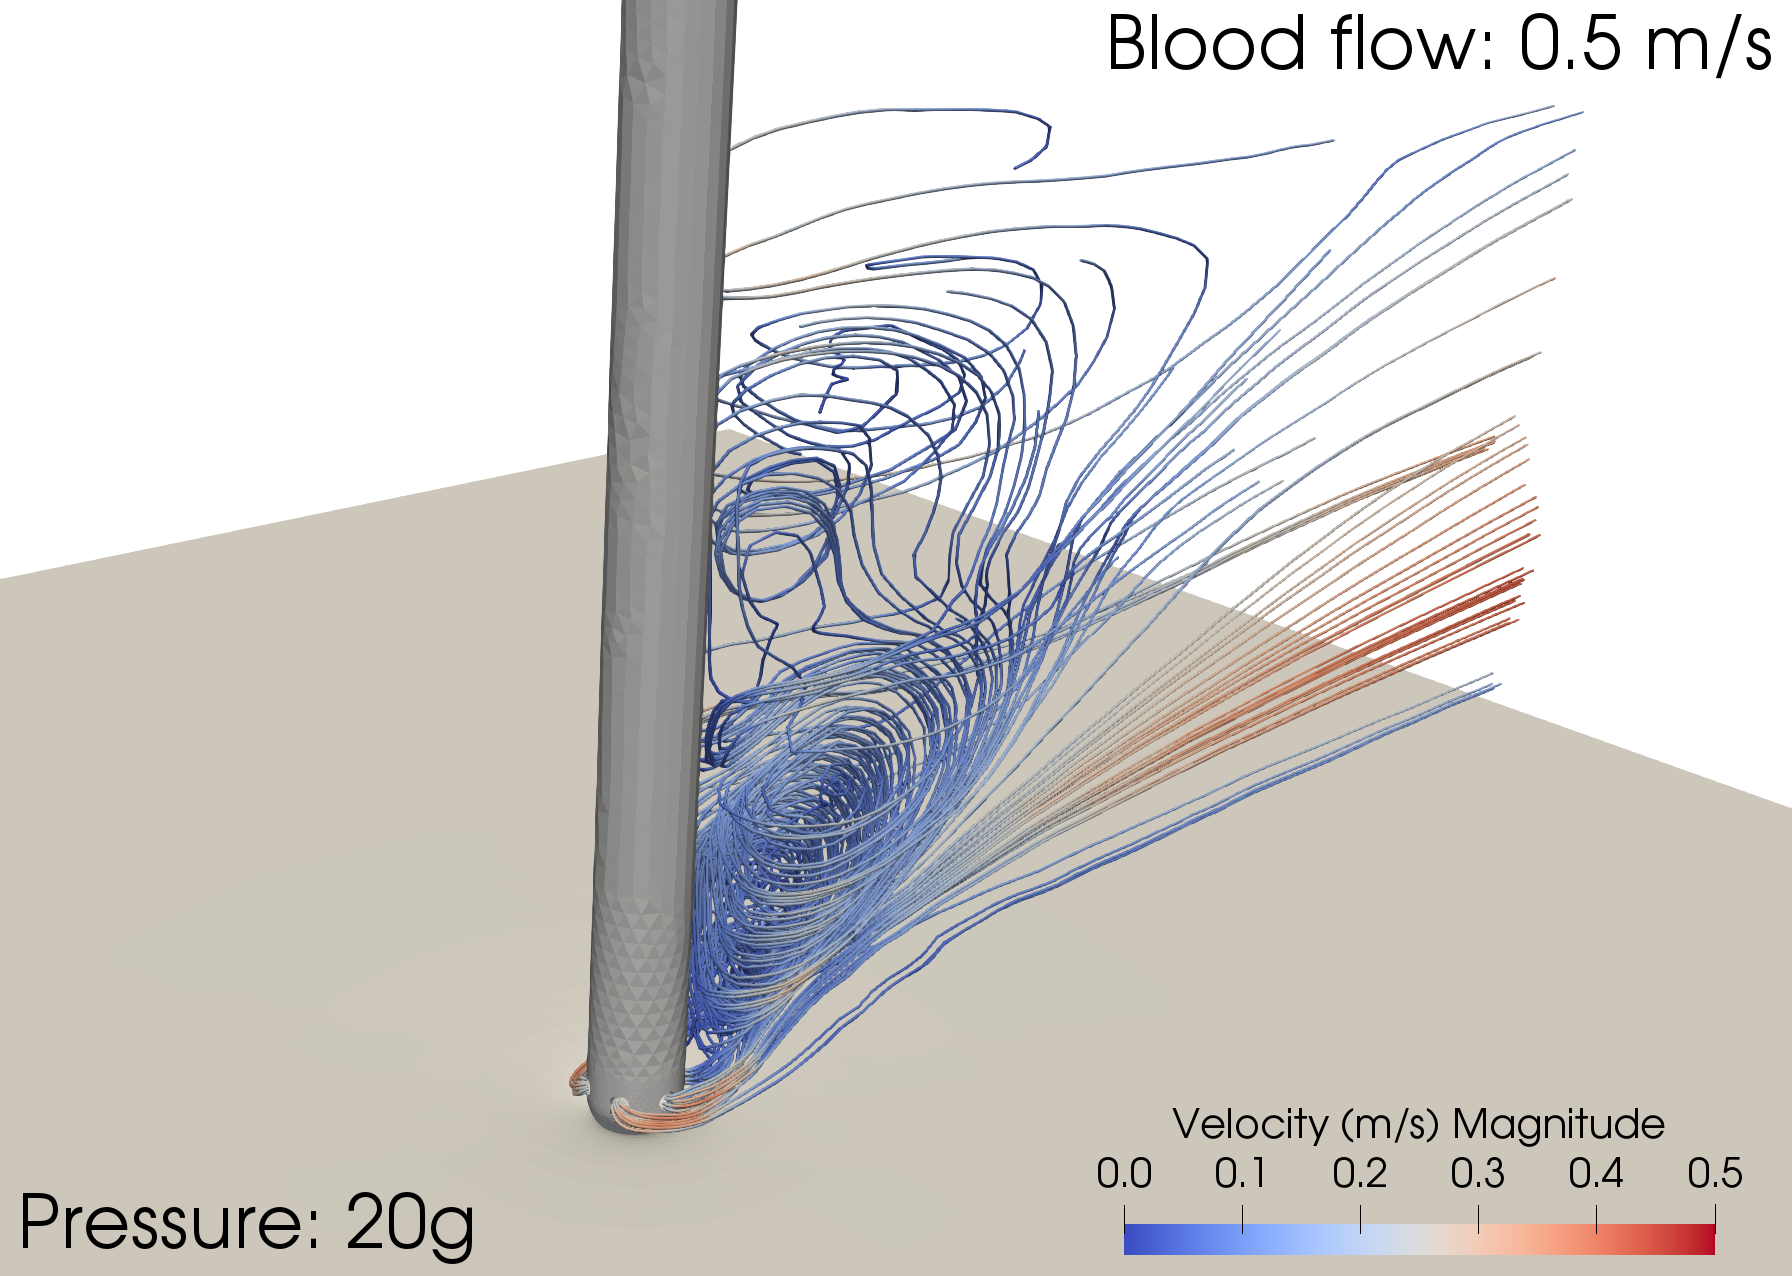
\includegraphics[width=0.45\textwidth]{img/rfa/salineHighFlow}}
      \quad
      \subfloat[][Low flow\label{fig_rfa_salineLowFlow}]
      {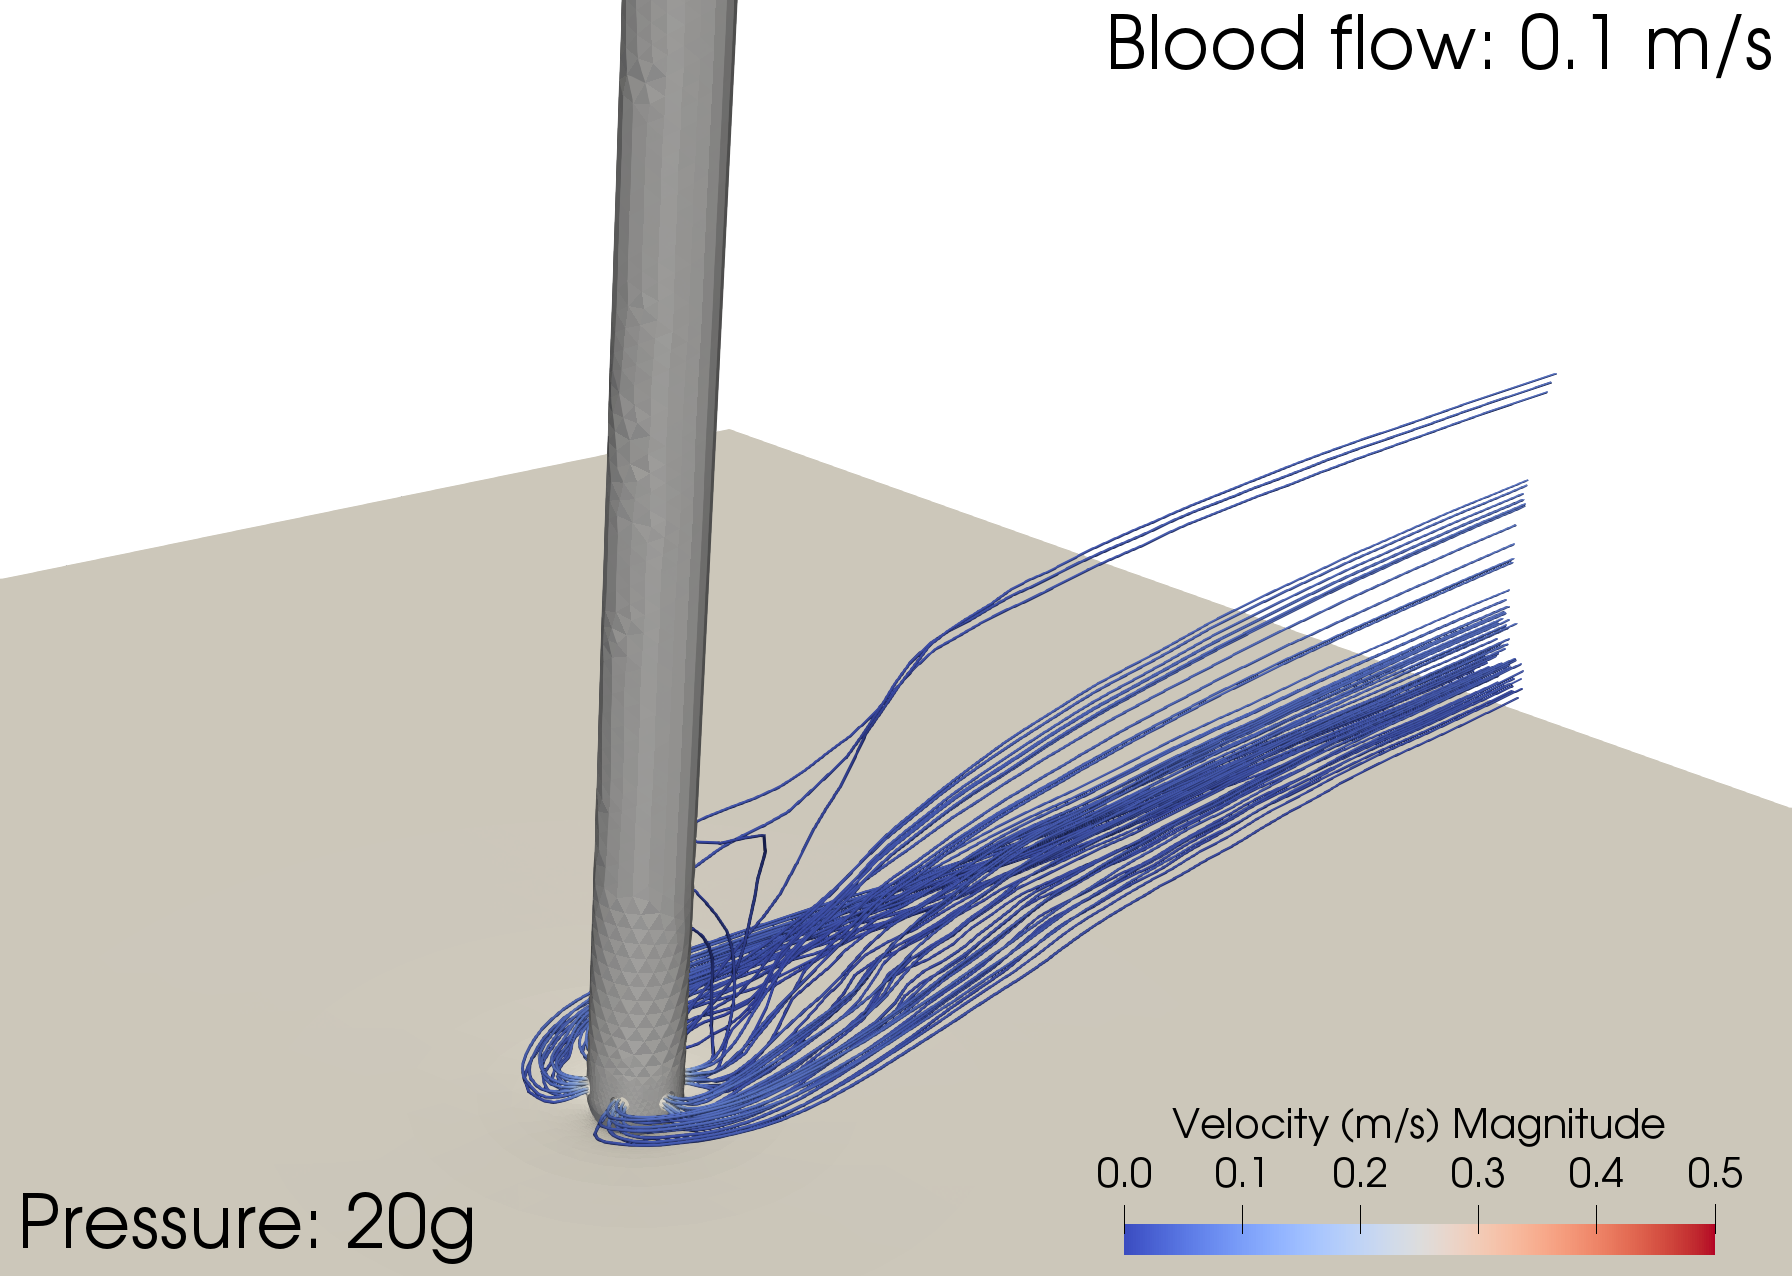
\includegraphics[width=0.45\textwidth]{img/rfa/salineLowFlow}}
      \caption{Convection of the saline coolant with a high flow (left) and a low flow (right) profiles.}
      \label{fig_rfa_saline}
    \end{figure}
    In Figure~\ref{fig_rfa_flowLesions} we show a comparison of lesions from simulations with high and low profiles, in front and lateral views.
    \begin{figure}
      \centering
      \subfloat[][High flow, front view.\label{fig_rfa_flowLesionsHX}]
      {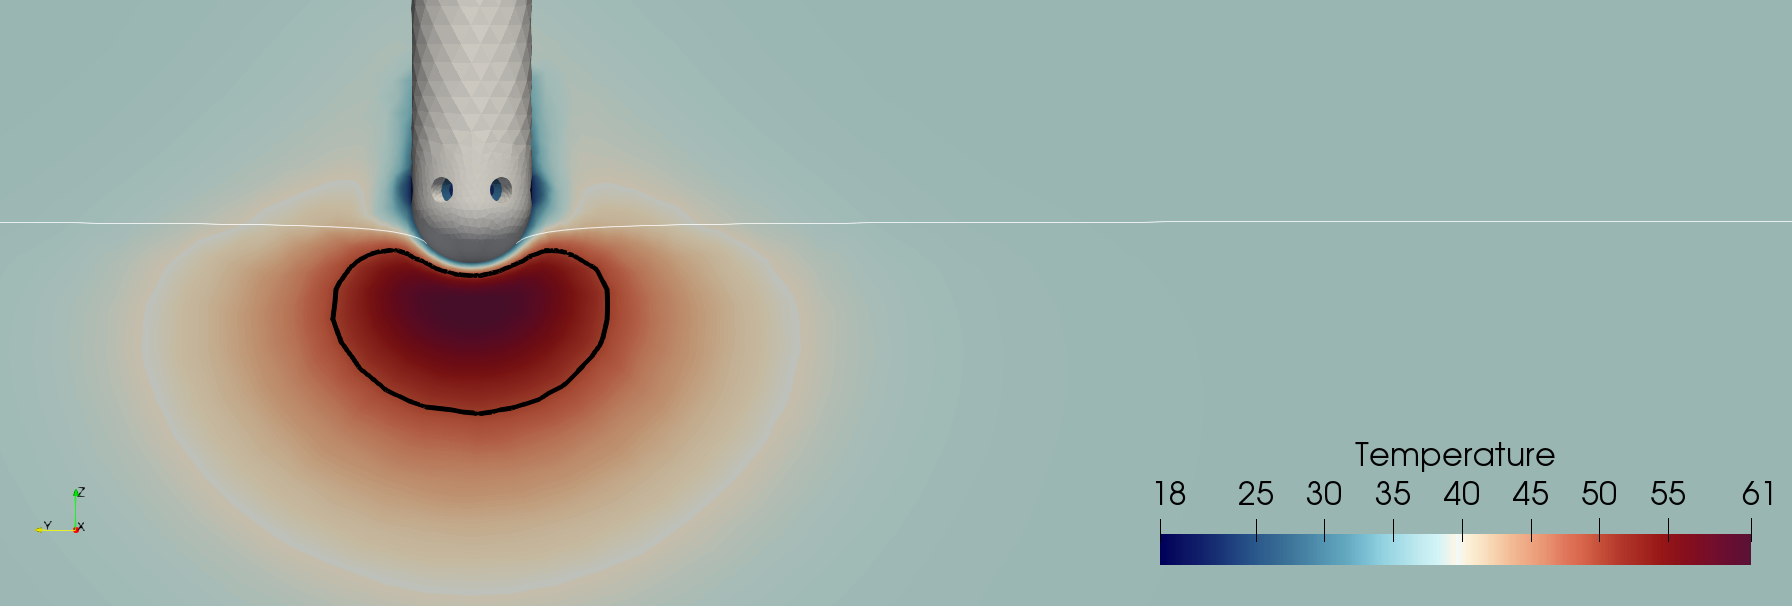
\includegraphics[width=0.45\textwidth]{img/rfa/HF_xaxis}}
      \quad
      \subfloat[][High flow, lateral view.\label{fig_rfa_flowLesionsHY}]
      {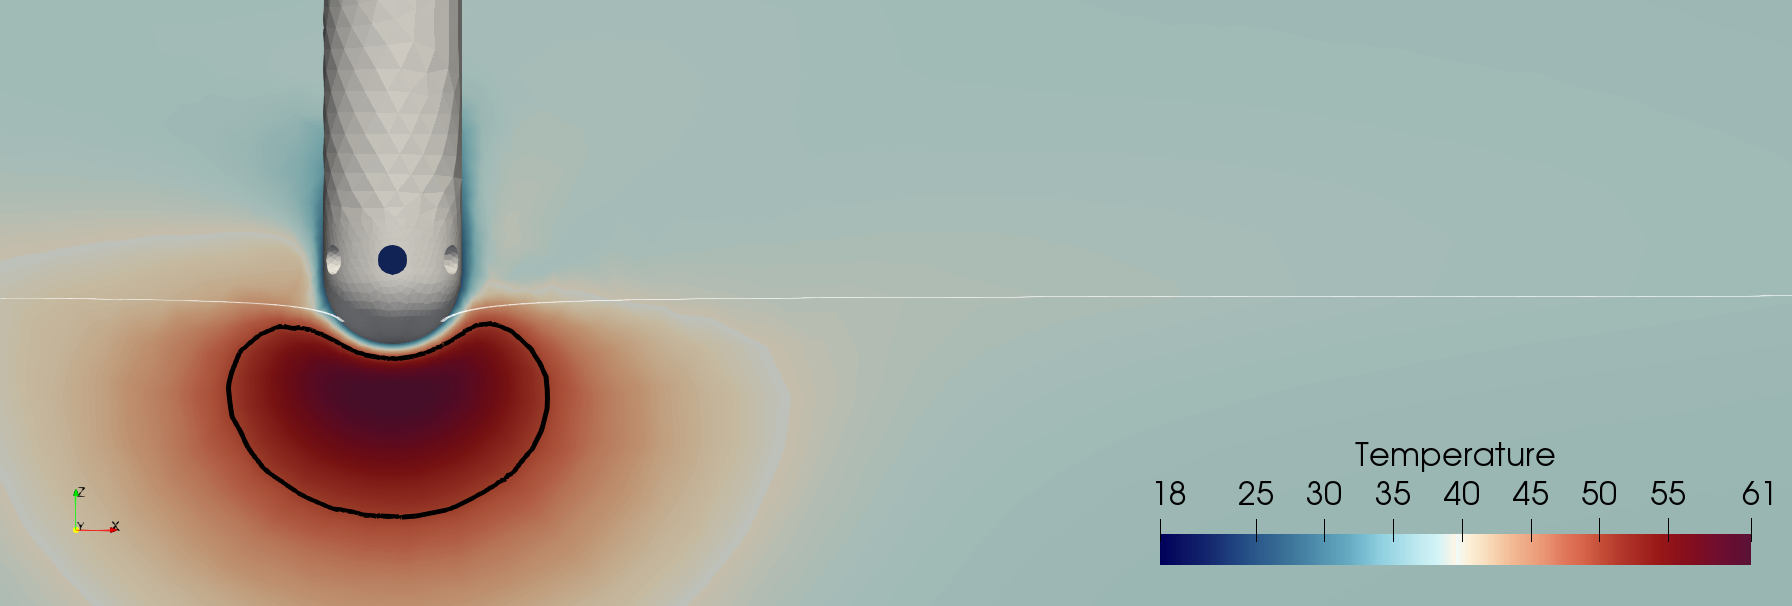
\includegraphics[width=0.45\textwidth]{img/rfa/HF_yaxis}}
      \\
      \subfloat[][Low flow, front view.\label{fig_rfa_flowLesionsLX}]
      {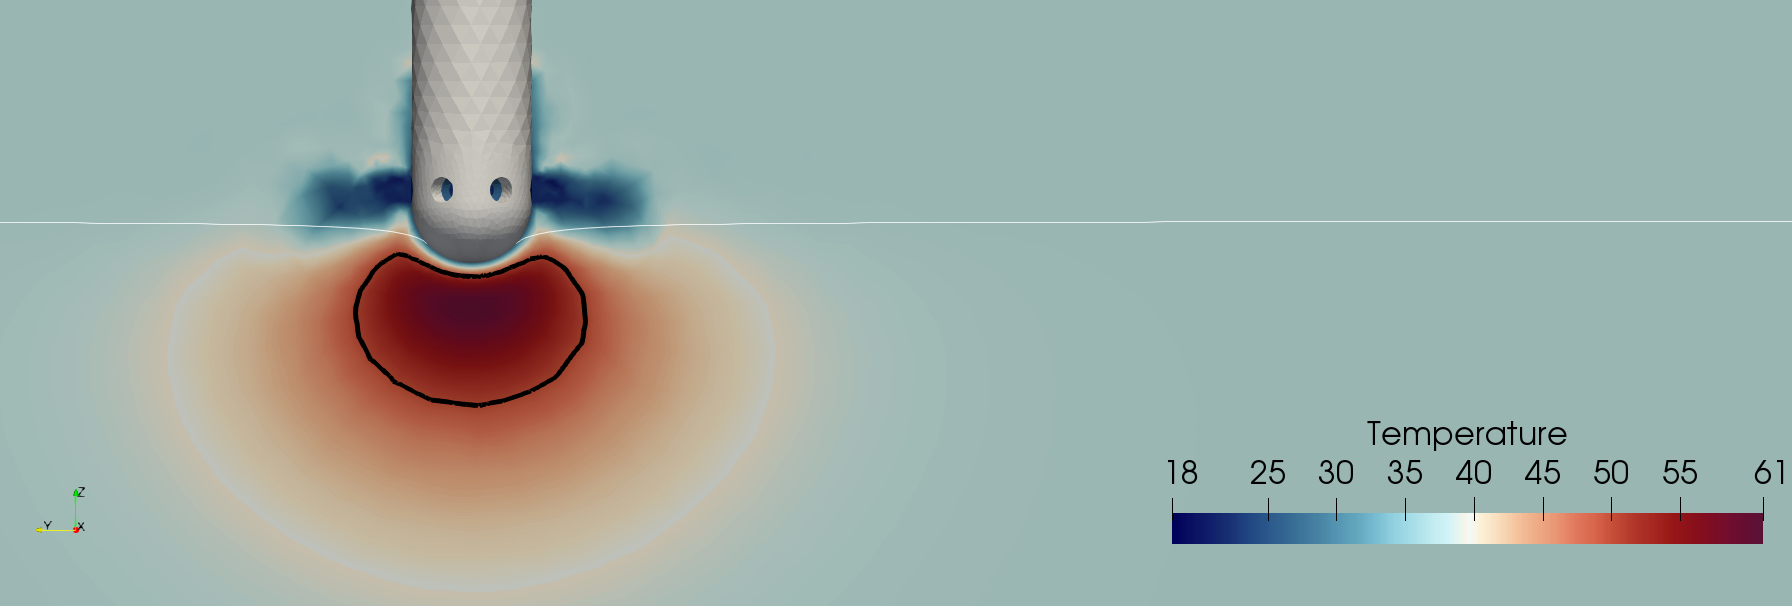
\includegraphics[width=0.45\textwidth]{img/rfa/LF_xaxis}}
      \quad
      \subfloat[][Low flow, lateral view.\label{fig_rfa_flowLesionsLY}]
      {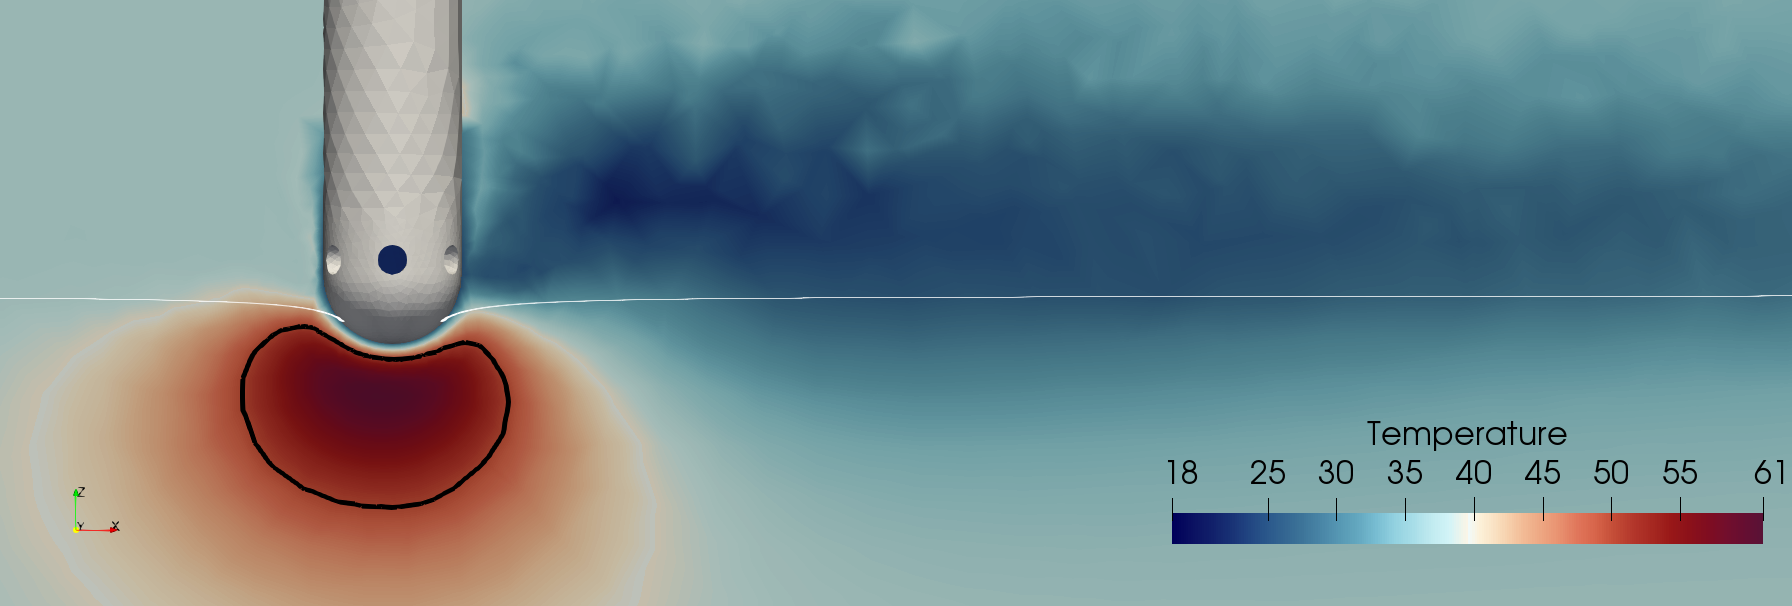
\includegraphics[width=0.45\textwidth]{img/rfa/LF_yaxis}}
      \caption{Lesion comparison with high and low flow profiles.}
      \label{fig_rfa_flowLesions}
    \end{figure}
    Interestingly, a low blood flow makes the coolant more effective as the lesion is overall smaller (Figure~\ref{fig_rfa_flowLesionsHX} versus Figure~\ref{fig_rfa_flowLesionsLX}) and asymmetric, as the cooling becomes more effective in the wake of the cylinder where the coolant stagnates a little longer (Figure~\ref{fig_rfa_flowLesionsHY} versus Figure~\ref{fig_rfa_flowLesionsLY}).
  \item \textbf{High-power ablation.} Recently, clinicians showed a lot of interest for \emph{high-power} ablation protocols, meaning protocols that prescribe ablations dissipating powers in the range \SI{70}{W}-\SI{90}{W}, significantly higher than what is common at the time of writing, but for shorter periods of time. The benefits would include reduced discomfort for the patient, from a shorter procedure, and in general a shorter time window in which complications can arise. We have been experimenting with high-power ablation protocols using our model, collecting results that we will present in an upcoming publication. Again, this only meant changing a number in our configuration and running several simulations.
  \item \textbf{Human versus animal tissue.} The experiments we reproduced were performed on porcine cardiac tissue. However, human cardiac tissue has different mechanical properties and, a priori, it is not clear if the results will be the same in terms of lesion sizes and maximum temperatures. Our model lets us verify this assumption very easily by simply setting different material properties for the tissue, resulting in a different electrode-tissue contact deformation, a parameter to which the simulation results are very sensitive, as we discussed. We collected results on this issue in a scientific contribution that is attached in the second part of this thesis.
\end{itemize}

The list above is not exhaustive and hopes to express the relevance of the model that we implemented and the number of research directions it allows us to investigate.



  \part{Papers}

  \backmatter
  \printbibliography[heading=bibintoc]

\end{document}
